\part{Introduction to the translation}




\chapter{Introduction to the translation}\label{chapter:HossepIntro}


\section{Introduction}

 

Armenian is an Indo-European language. Its oldest attested form is Classical Armenian (CA). The modern language is conventionally described as having two standardized variants: Standard Western Armenian (SWA or WA) and Standard Eastern Armenian (SEA or EA). Alongside these two varieties, there are countless non-standard dialects, many of which were were made extinct because of the Armenian Genocide. 

This book is an English translation of a monograph originally written in Armenian by Hrachia Adjarian \citep{Adjarian-1911-DialectologyBook}: ``\armenian{Հայ Բարբառագիտութիւն}'' or ``Armenian dialectology''. The original monograph consisted of descriptions of 31 non-standard Armenian varieties. Some descriptions are rather lengthy, while some are short.  Of course, more non-standard varieties exist that weren't described in this monograph  \citep{GreppinKhachaturian-1986-HandbookArmenianDialectology,Martirosyan-2019-Armeniandialects,Martirosyan-2019-ArmenianDialectsBigVersionRussianJournal,DolatianEtAl-prep-IranianGrammar}.

The present book is both a translation and commentary on this monograph. In the course of translating the original 300-paged book into English, I had to unpack a lot of implicit knowledge that Adjarian was using in order to describe the varieties. For example, Adjarian did not use morpheme boundaries, glosses, nor IPA symbols. He would often just provide data points from a dialect, with a brief prosaic description and with cognates from Classical Armenian. That brief description relied on the reader's knowledge of Standard Armenian (and sometimes Classical Armenian) in order to deduce the linguistic structure of the non-standard dialect. In order to unpack this implicit information, the end result was a 700-paged translation, with glossing, translation, and morpheme segmentation.


The current introduction is written by myself, the translator. The rest of this book is my translation of Adjarian's writing. At times, I have to provide commentary and interrupt Adjarian's prose. To prevent ambiguity, I wrote my interruptions in the following format:

\begin{center}
	\translatorHD{This is an interruption by the translator, Hossep Dolatian.}
\end{center}

To maximize the recoverability of information during the translation, I provide the page numbers from Adjarian's original monograph. 

The rest of this chapter provides basic information on Armenian (\S\ref{sec:HossepIntro:armenian}), my transcription system (\S\ref{sec:HossepIntro:phonotransc}),   and my translation conventions (\S\ref{sec:HossepIntro:translation}).



\section{Armenian linguistics and dialectology}\label{sec:HossepIntro:armenian}


This section provides basic information on what is the Armenian language. This section is geared to summarize basic diachronic and synchronic facets of the Armenian language in terms of how we categorize different Armenian varieties. I first explain the history of the langauge (\S\ref{sec:HossepIntro:armenian:whatisarm}). I then focus on the nature of the two standardized modern varieties  (\S\ref{sec:HossepIntro:armenian:whatisarm}), the non-standardized varieties (\S\ref{sec:HossepIntro:armenian:whatisdialect}), and the classification or genetic relationship across   varieties (\S\ref{sec:HossepIntro:armenian:whataredialect}). Adjarian's dialectological maps are provided in \S\ref{section:HossepIntro:maps}.  
\subsection{What is Armenian}\label{sec:HossepIntro:armenian:whatisarm}

As stated, Classical Armenian is the oldest attested Armenian variety (circa the 5th century CE).\footnote{To clarify, CA was first attested in the 5th century in written form in a Bible translation. Before this initial attestation, we don't know what was the linguistic situation for Armenians. It is often assumed that were a stage of Proto-Armenian between Proto-Indo-European and Classical Armenian. } In contrast, Modern Armenian is conventionally described as having two standardized variants: Standard Western Armenian (SWA or WA) and Standard Eastern Armenian (SEA or EA). These two variants are often also called just Western Armenian and Eastern Armenian. 

Between the ancient centuries of Classical Armenian and the modern century of Standard Western/Eastern Armenian, ther are many holes. We know that there was a stage of Middle Armenian during the medieval period. However, Middle Armenian is less described or studied than either the Classical or Modern forms \citep{Karst-1901-MiddleArmenain}. 

By sometime in the 18th century, ethnic Armenians spoke a variety of languages. As Adjarian describes in \S\ref{chapter:NonSpeaking}, some groups of Armenians spoke only non-Armenian languages like Turkish. Other groups had developed their own individual Armenian varieties. Thus the Armenians of Smyrna (in modern Turkey) spoke Smyrna Armenian, while the Armenians of Julfa (in modern Iran) spoke Julfa Armenian, and so on. These different language varieties had enough structural differences to treat them as different linguistic objects. 

Just as there are two geogrpahically-defined modern standard forms (Western Armenian and Eastern Armenian), these region-specific dialects are conventionally divided into two branches. Some dialects like Symrna belong to the Western branch (and are more similar to Western Armenian than to Eastern Armenian). While some dialects like Karabakh/Artsakh belong to the Eastern branch. 

Alongside these region-specific varieties of Armenian, the early modern period (17/18th centuries) showed the rise of an Armenian lingua franca among Armenians \citep{Parnassian-1985-FormationAshkharabar,Donabedian-2018-WestArmTypoSocio}. This lingua franca or koine was Civil Armenian (Ashkharhabar or \armenian{Աշխարհաբար} [ɑʃχɑɾɑbɑɾ, ɑʃχɑɾɑpʰɑɾ]). It is often seen as some sort of amalgamation of various linguistic features from different regions. This lingua franca developed in two sets of cultural centers: Istanbul in the West, and Yerevan and Tbilisi (Tiflis) in the East. 

The outcome of Civil Armenian was establishing two separate standardized Armenian varieties: Standard Western Armenian (SWA) and Standard Eastern Armenian (SEA). The two dialects are often treated as developed from Istanbul Armenian and Yerevan Armenian via a process of standardizing the lexicon, removing recent Turkic borrowings, and incorporating common dialectal features. For example, \citet{Manoukian-2022-LiteraryTranslationExpansionOttomanArmenian} tracks the development of SWA within publishing houses in the Ottoman Empire in the 19th century. She describes how the translators developed a `purified vernacular' language that removed Turkish words, and replaced them with Classical Armenian words or calques. 

However, there are non-trivial structural differences between the non-standard sources and the standardized derivatives \citep{SayeedVaux-2017-EvolutionArmenian}. These differences make it difficult to be sure of the exact genetic relation between Istanbul Armenian and SWA, and between Yerevan Armenian and SEA. For example, there are structural differences between SWA and the Istanbul Armenian of 1911 (\S\ref{chapter:istanbul}), and these difference make it unclear whether SWA is a simplified descendant of Istanbul vs. a sister dialect \citep[1148]{SayeedVaux-2017-EvolutionArmenian}. We talk about some of these differences in the next section. Adjarian himself suggests that SWA may have developed by combining grammatical aspects of Istanbul Armenian with some phonological aspects of other dialects such as Rodosto Armenian (\S\ref{section:Rodosto:Phono:SoundChange:Laryngeal}). This suggests that SWA developed as a form of dialect leveling across multiple dialects, and not as a simple descendant from only one dialect. 

In terms of what we know about the linguistic situation of Armenians in the 19th century, we owe a great debt to Hratchia Adjarian. Within Armenian linguistics, a pioneering researcher was Hratchia Adjarian (Armenian: \armenian{Հրաչեայ Աճառեան}, reformed spelling; also transliterated as Acharian). He was born in modern Istanbul in 1876, and undertook an education in linguistics in France. In French, his two most groundbreaking works were \citet{Adjarian-1899-ArmenianExplosives} where he developed an experimental procedure for Armenian consonant acoustics, and discovering an early form of voice onset time \citep{braun-2013-earlyCaseVOTAdjarian}. His second major was \citet{Adjarian-1909-ClassificationArmenianDialect} ``Classification des dialectes arméniens'' (``Classification of Armenian Dialects'') where he catalogued, described, and classified a set of Armenian varieties. This French monograph was then the basis for a larger work in Armenian \citep{Adjarian-1911-DialectologyBook}: ``\armenian{Հայ Բարբառագիտութիւն}'' or ``Armenian dialectology''. These manuscripts provide some of the few detailed microscopes into the linguistic reality of early modern Armenians. 

Thus, by the time of Adjarian's monograph in 1911, there were a large number of living forms of Armenian: SEA, SWA, Istanbul Armenian, Yerevan Armenian, and a host of other area-specific Armenian varieties. Unfortunately, since 1911, the linguistic landscape of Armenian populations has significantly changed. The vast majority of non-standard dialects are now extinct or moribund. Some dialects were made extinct because of the Armenian Genocide \citep{Katvalyan-2015-GenocideArmenianLanguage}; Smyrna is a potential example \citep{Vaux-2012-ArmenianSmyrna}. Some of these dialects survived the Genocide, but its speakers underwent language shift to one of the standard varieties. For example, the Shamakhi dialect was spoken in Shamakhi in modern-day Azerbaijan. But because of Azerbaijani persecution, the Armenian populace of Shamakhi has been migrating to Armenia, and the community has been undergoing language shift to SEA \citep{Vlasyan-2019-Shamakhi}. 

In contrast, it is relatively rare to find Armenian communities that still speak a non-standardized dialect. Many are endangered, but there are still pockets of Armenian communities that speak and transmit these non-standard dialects.  Because of various wars in the 19th-20th centuries and the Armenian Genocide, various dialect communities have settled in the modern Republic of Armenia and Georgia (\citealt[\S2.2.2]{Hodgson-2019-DissRelativeClauseArmenianSyntax}). These communities are in continuous pressure from SEA, but they some of them are currently viable (Hodgson, p.c.). In Georgia and Abkhazia, there    large communities of Karin/Erzurum and Hamshen speakers, and their langauge maitenance also seems viable \citep{Bezrukov-2022-DissCaucasusMotionArmenian}.  A very viable community is the Armenian community in Tehran, Iran, who have developed and maintained their own dialect of Tehrani Iranian Armenian \citep{DolatianEtAl-prep-IranianGrammar}, which is surprisingly absent from Adjarian's work. One could argue that some of the traditional dialects of Cilicia (\S\ref{chapter:Cilicia}) and Syria (\S\ref{chapter:Syria}) are still spoken in a handful of villages in the Middle East (Kessab, Anjar, Vaqif). But the communities are small and caught in dangerous circumstances (such as the Syrian war); thus they may be considered endangered.

 The present monograph is an attempt to preserve information on many of these lost languages. The above is a basic conventional summary of how Armenian varieties work. But there are some points of nuance that we should clarify. The next sections discuss these points. 

 

\subsection{What is Standard Armenian?}\label{sec:HossepIntro:armenian:whatisstandard}
The term `standard' in the name `Standard Western Armenian' does not denote a literary variety that's limited to books and formal speech. For the majority of Western Armenians who speak some Armenian variety, that variety is Standard Western Armenian. Similarly, Standard Eastern Armenian is the native language of the majority of Eastern Armenians. The confusing use of the term `standard' is caused by patterns of language shift and dialect leveling among Armenians.

For example, in 1911, the year that the Adjarian monograph was published, the Armenians of Istanbul spoke a specific variety of Armenian called Istanbul Armenian. This variety is documented in this book in chapter \S\ref{chapter:istanbul} and also later by Adjarian in a separate \citep{Adjarian-1941-IstanbulDialect}. The variety of Istanbul Armenian in 1911 (and its 1941 followup) is not identical to SWA. The following are some subtle differences that I've noticed. 

\begin{itemize}
	\item Differences between SWA and Istanbul Armenian
	\begin{enumerate}
		\item The word for `father' is [hɑjɾ] <\armenian{հայր}> in SWA; but Adjarian describes the Istanbul form as [hɑɾ] <\armenian{հար}> (\S\ref{sec:Istanbul:phono:soundchange:diph}).
		\item The reflex of the Classical Armenian sound /d͡z/ <\armenian{ձ}> in Istanbul is /d͡z/ <\armenian{ձ}>, while its reflex in SWA is /t͡sʰ/ <\armenian{ց}> (\S\ref{sec:Istanbul:phono:soundchange:cons:laryngeal}). For example, the word `snow' <\armenian{ձիւն}> is /d͡ziu̯n/ in CA, /d͡zun/ in Istanbul, but /t͡sʰʏn/ in SWA (Table \ref{tab:Istanbul:phonology:change:dipth}). Adjarian himsels notes this contrast in \S\ref{sec:Istanbul:phono:segment:vowel}. 
		\item The reflex of the Classical nominalizer <\armenian{ութիւն}> /-utʰiu̯n/ `-ation' is /-utʰʏn/ in SWA, but /-utʰin/ in Istanbul (\S\ref{sec:Istanbul:morpho:noun}). 
		\item The causative suffix is /-t͡sʰənel/ <\armenian{ցնել}> in SWA but /-t͡sʰunel/ in Istanbul. For example, `to make live' is /ɑbɾe-t͡sʰənel/ in SWA (\armenian{ապրեցնել}) but /ɑbɾe-t͡sʰunel/ in Istanbul (\armenian{աբրէցունէլ}) \citep[140]{Adjarian-1941-IstanbulDialect}. 
	\end{enumerate}
\end{itemize}






Although Adjarian does not discuss the sociolinguistic situation of this community in depth, we suspect that this variety was acquired by Armenian children at home. At school, they would learn Standard Western Armenian, so that they could read, write, and engage with other Armenian communities as a lingua franca. 

Since 1911 however, the Istanbul community has shifted from using the Istanbul dialect to using SWA. As a member of the Istanbul Armenian community, Tabita Toparlak reports that the dialect described by Adjarian has died out. Instead, Armenian-speaking families have shifted to using SWA at home. 




A similar situation is described for SEA and Yerevan. In the time of Adjarian 1911, the dialect of Yerevan had a distinctive feature of penultimate stress (\S\ref{sec:Yerevan:phono:stress}). In contrast, SEA has final stress. But in the decades since, the community in Yerevan has shifted towards using SEA and not the old Yerevan dialect. A native of this city (Vahagn Petrosyan) reports the following:

\begin{quote}
	[The] ``Yerevan dialect'' is a historical label. Currently Yerevan speaks a colloquial version of Standard Eastern Armenian.
	
	I have heard the features described for this dialect in the speech of some Yerevan residents. For me the speech is associated with the [lower classes]. I don't know if these people are recent migrants from villages of the Ararat dialect areas or if they are the remnants of the original Yerevan dialect speakers. In any case, an average person certainly does not grow up speaking like that. I am from Yerevan and I speak normally. 
\end{quote}

Thus, the majority of the dialects in Adjarian 1911 are likely extinct, due to either genocide or language shift. For the standard varieties (SWA and SEA), these are not fossilized variants restricted to books. They are the native language of most Armenian-speaking children and adults. They are not simplified forms or daughters of past Armenian varieties (Istanbul or Yerevan), but they are their own distinct Armenian varieties that are natively acquired and used.\footnote{This situation is similar to the development of Italian. The language developed from Tuscan, and was standardized. The language then became a state language, and spread throughout Italy. As another helpful analog, the sitaution with SWA/SEA is not like Arabic diglossia. For Arabic, the standard written form (Modern Standard Arabic) is not the home langauge of any Arabic-speaking household; the home language is instead one of many Arabic dialects like Levantine or Egyptian. }





Of course, like any spoken language, SWA has both informal and formal registers. The informal register is acquired at home, while the formal register is taught at schools or acquired via formal interactions. The two registers have minor differences. Some traits of the informal register of SWA is found in various non-standard dialects. For example, informal spoken SWA uses a progressive marker [ɡoɾ], while formal written SWA bans this marker \citep{donabedian-2001-tabouLinguisticArmenianOccidentalGorProgressive}. The use of [ɡoɾ] is likewise found across various non-standard Western dialects such as Istanbul. Similarly, SEA has both formal and informal registers. The 3SG auxiliary `is' is pronounced [e] in formal SWA, but pronounced [ɑ] in informal SEA. The use of an auxiliary [ɑ] is again found in non-standard Eastern dialects like Yerevan (\S\ref{sec:Yerevan:morpho:verb:morphodetials:copula}). For a sample of other informal vs. formal register differences, see elsewhere (\citealt{Gharagyulyan-1981-ColloquialArmenian,Zakaryan-1981-ColloquialArmenian,Aghayan-1981-ColloquialArmenian,Kavassian-1983-CertainProblemMorphologyArmenianMontreal,DumTragut-2009-ArmenianReferenceGrammar}, \citealt[ch3]{Karapetian-2014-TeachArmenianEasternArmenianHeritage}).


Thus the presence of the word `standard' in the names `Standard Eastern Armenian' or `Standard Western Armenian' does not indicate prescriptivism, but is due to the history of the emergence of these standardized varieties. Because of this history, names like `Standard Western Armenian' and `Western Armenian' are interchangeable. In my experience, in Armenian linguistics, it is common to add the word `standard' in order to disambiguate terms like `Western Armenian' which could designate either a single variety (Standard Western Armenian) or an entire branch of dialects (Western dialects). 

In contrast, the term `Standard Western Armenian' can mean either `the formal register of Western Armenian' or `either the formal or informal register of Western Armenian.' In my case, I grew up in an Armenian-speaking household in Lebanon. I acquired the informal register of (`Standard') Western Armenian. My idiolect does not correspond to any of the non-standard varieties like Smyrna, Trabzon, or Crimea. I then learned the formal register `Standard' Western Armenian at school. 









\subsection{What is a dialect?}\label{sec:HossepIntro:armenian:whatisdialect}

The original Armenian monograph from 1911 was called ``Armenian dialectology'', based on an expansion of a French monograph from 1909 called ``Classification of Armenian dialects.'' This section clarifies the term `dialect'. 

In linguistics, a common criterion for labeling a language variety as a dialect is mutual intelligiblity. Given two language varities A and B, if a speaker of A can easily understand a speaker of B, then the two varities are dialects of the same language. Based on this criterion, American English and British English are dialects of English. 

For Armenian however, the various varieties are conventionally called `dialects', but they are not mutually intelligible. For example, as a speaker of SWA, I have difficulty fully understanding a spoken SEA sentence due to my limited exposure to spoken SEA. Written SEA is however quite intelligible to me. Thus, I often hear among lay speakers of Armenian that the two dialects are mutually intelligible after significant exposure. 

For the non-standard dialects, mutual intelligibility is much weaker. For example, this monograph has text samples for each of the 31 non-standard dialects. I could not translate any of them because I couldn't understand them. The best I could understand were the Istanbul texts, but I was not confident enough to provide an actual translation, morphological segmentation, or glossing. 


Thus based on the criterion of mutually intelligibility, Standard Armenian (SEA and SWA) and the various non-standard varieties (Julfa, Tigranakert, and so on) are mutually unintelligible and not dialects of the same language. Because of mutually unintelligibility, some linguists go so far to use the term `Armenoid' to describe the different Armenian varieties, e.g., that Agulis is an Armenoid language \citep{Vaux-2008-ArmenianZok} and not an Armenian dialect (\S\ref{chapter:Agulis}). 

In Armenian studies however, all these language varieties are just called `dialects'. The term is used in a non-theoretical stance. I suspect that because all these Armenian varieties are spoken by ethnic Armenians, then the term `dialect' is used to indicate ethnic solidarity. To reduce confusion, I will also use the term `dialect' in this translation, simply because Adjarian himself was using the Armenian word for dialect: [bɑɾbɑr, pʰɑɾpʰɑɾ] <\armenian{բարբառ}>. In my own commentaries, I will often use the terms `dialect' and `variety' interchangeably. 





\subsection{What are the dialects?}\label{sec:HossepIntro:armenian:whataredialect}

In Armenian dialectology, dialects are commonly divided into two branches: Western and Eastern. We discuss some controversial choices that Adjarian made in his classification. 


As said before, Classical Armenian is the oldest attested Armenian variety. Modern Armenian varieties are conventionally divided into groups: Western dialects and Eastern dialects. In general, the division between dialects is based on geographic origin. The division (imperfectly) corresponds to the modern Turkey-Armenia border. Armenian varieties that developed west of this border (in the Ottoman Empire) belong to the Western branch, while varieties that developed to this east of this order (in the Russian/Persian empires) belong to the Eastern branch. 

For example, SWA developed in Istanbul, while SEA developed in Tbilisi and Yerevan. SWA and SEA are conventionally treated as standardized offshoots of Istanbul and Yerevan. This basic classification is summarized in Figure \ref{tree:dialect:basic}.\footnote{For easier illustration, I don't include Middle Armenian here. And as said before, we don't know with complete certainty whether SWA (SEA) is a descendant of Istanbul (Yerevan) vs. a separate development from multiple dialects or from Civil Armenian. For easier illustration, the figures in this section treat the standard dialects as descendants. }

\begin{figure}[H]
	\caption{Conventional and simplified family tree of Armenian}
	\label{tree:dialect:basic}
	\resizebox{\textwidth}{!}{%
\begin{forest}
[{Classical Armenian} [Western [... ] [Trabzon ] [Crimea ] [Istanbul [{Standard Western}] ] ] [Eastern [Yerevan [{Standard Eastern}] ] [Julfa] [Agulis] [...] ] ]
\end{forest}
}
	\end{figure}

 
The above simple classification correlates with an important islogloss in Armenian dialectology: the morphemes used to form the indicative present (Table \ref{intro:tab:ea wa ia differences: morpho}) \citep{Vaux-1995-ArmenianVerbDiachrony}. In Classical Armenian, the indicative present was formed by adding agreement suffixes directly onto to the verbal stem. The verb stem consists minimally of a root and theme vowel. But in modern SEA and SWA, this simple synthetic construction is instead used for the subjunctive present. To form the indicative present, SWA adds a prefix /ɡə/ <\armenian{կը}> before the synthetic form. In contrast, SEA uses a periphrastic or analytic construction. The verb is a non-finite form called the imperfective converb. The verb takes the non-inflecting suffix /-um/, while agreement is on an auxililary. 

\begin{table}[H]
	\caption{Morphemes used for the indicative present in CEA, SWA, and SEA}\label{intro:tab:ea wa ia differences: morpho}

%		\ex 
		\centering
		\begin{tabular}{|l| ll|}
			\hline 	& \multicolumn{2}{l| }{Indicative present `I like' } \\
		\hline 	CA & siɾ-e-m& like-{\thgloss}-1{\sg}\\
			SWA & ɡə-siɾ-e-m&{\ind}-like-{\thgloss}-1{\sg}\\
			SEA & siɾ-um e-m& like-{\impfcvb} {\aux}-1{\sg}\\
			\hline 
		\end{tabular}

\end{table}

The above parameters (geographical and morphological) are foundational to Armenian dialectology.\footnote{Other       major and theoretically-interesting parameters of variation are also attested, such as voice onset time or voicing differences (\citealt[\S1.1.1]{Vaux-1998-ArmenianPhono}; \citealt{Baronian-2017-TwoProblemsArmenianPhono}), vowel harmony \citep{Vaux-1998-ArmenianPhono}, stress \citep{DeLisi-2018-ArmenianProsodyDiachrony}, mobile affixes or ambifixies \citep{BezrukovDolatian-2020-PLCArmenianMobile,Bezrukov-2022-DissCaucasusMotionArmenian}, auxiliary movement \citep{Comrie-1984-SomeFormalPropertiesFOcusEasternArmenian,KahnemuyipourMegerdoomian-2011-secondcliticvP,KahnemuyipourMegerdoomian-2017-positionalDistriutionFocus}, auxiliary-induced phonosyntactic processes \citep{DolatianEtAl-prep-IranianGrammar}, relative clause formation \citep{Hodgson-2019-DissRelativeClauseArmenianSyntax}, and so on.} These two parameters however  have some problems. 

For the geographical parameter, the terms `Western' vs. `Eastern' refer to the ultimate geographic origin of some Armenian variety. But as Adjarian describes in \S\ref{sec:ThreeBranch:overview}, this geographic parameter can be confusing when we take into account migration patterns. For example, the dialect of Karin (\S\ref{chapter:Karin}) is a Western dialect that historically developed in what is now modern Erzurum (in modern eastern Turkey). But during the 19th century and after the Armenian Genocide, the Armenian community of Erzerum had migrated to what is now modern Armenia and Georgia. That is, this Western community moved from west of the Turkey-Armenia border to the east of this border. For Karin, it is thus somewhat confusing call this dialect a Western dialect, even though it is geographically spoken on the east of the relevant geographic border. 

Because of the above geographical problems, Adjarian argued that descriptions like `Western' vs `Eastern' branches should be replaced with terms based on isoglosses. The most obvious isogloss for Adjarian was the morphology of the indicative present. He specifically argued that `Western' dialects (like SWA) belong to the /kə/ <\armenian{կը}> branch, while `Eastern' dialects (like SEA) belong to the /um/ <\armenian{ում}> branch.\footnote{Note that Adjarian used the term /kə/ branch instead of /ɡə/ branch. Although the indicative prefix is /ɡə/ in SWA, this prefix is spelled <\armenian{կը}>. The ancestor of this prefix is pronounced as /kə/, such as in SEA where this prefix is used to mark the conditional future.}

In addition to replacing geographic descriptions with morphological ones, Adjarian also argued that some dialects belong to a third separate branch. This branch is called the /el/ <\armenian{էլ}> branch and includes dialects like Maragha (\S\ref{chapter:Maragha}). For such dialects (\S\ref{sec:Maragha:morpho:verb:overview}), the indicative present is formed by adding an auxiliary after the infinitive. The construction is periphrastic, and the surface [el] sequence is actually the theme vowel /-e-/ plus the infinitive suffix /-l/ (\ref{sent:Maragha:morpho:verb:infconj:merged}). 

\begin{exe}
		\ex Maragha (taken from \ref{sent:Maragha:morpho:verb:infconj:merged})
\\
	 \gll ʏz-e-l-i-m \\
			want-{\thgloss}-{\infgloss}-{\aux}-1{\sg} \\
			\trans `I want.'\\
			\armenian{իւզէլիմ} \label{sent:Maragha:morpho:verb:infconj:merged REP in intro} 
			
	
\end{exe}

To summarize, Adjarian argues for a more detailed classification, as in Figure \ref{tree:dialect:adj}. 

\begin{figure}[H]
	\caption{Expanded family tree of Armenian based on Adjarian's classification}
	\label{tree:dialect:adj}
	\resizebox{\textwidth}{!}{%
			\begin{forest}
		[{Classical Armenian} [/kə/ branch [... ] [Trabzon ] [Crimea ] [Istanbul [{Standard Western}] ] ] [/um/ branch [Yerevan [{Standard Eastern}] ] [Julfa] [Agulis] [...] ] [/el/ branch [Maragha] [...] ] ]
	\end{forest}
}
\end{figure}

In contrast, in a simpler two-branch classification, the dialects of the /el/ branch would be considered Eastern dialects. First, dialects like Maragha were formed in modern-day Iran and Russia; thus they are geographically east of Turkey. Second, both /um/ branch and /el/ branch dialects utilize morphological periphrasis in forming the indiciative present. Thus, varieties like SEA and Maragha share a more abstract isogloss. Figure \ref{tree:dialect:compromise} shows a possible family tree by combining both geography and Adjarian's three branches. 

\begin{figure}[H]
	\caption{Family tree of Armenian based on geographic terms and Adjarian's /el/ branch}
	\label{tree:dialect:compromise}
	\resizebox{\textwidth}{!}{%
	\begin{forest}
		[{Classical Armenian} [{Western (/kə/ branch)} [... ] [Trabzon ] [Crimea ] [Istanbul [{Standard Western}] ] ] [Eastern [{/um/ branch} [Yerevan [{Standard Eastern}] ] [Julfa] [Agulis] [...] ] [/el/ branch [Maragha] [...] ] ] ]
	\end{forest}
}
\end{figure}
 
This book maintains Adjarian's original three-way classification system. I do this so that the translation is faithful to Adjarian's original intentions. However, since 1911, it seems that most dialectological work in the West has not replaced geographic terms with isogloss-based terms.\footnote{I personally think that abandoning geographic terms is unconvincing. Although it is true that some Western dialects like Karin are now spoken east of the Turkey-Armenia border, they still historically developed west of this border. What matters is a dialect's genetic relationships with other dialects, and geography is a major correlate of such genetic connections. } As for Soviet Armenia and the modern Republic, it seems that further dialectological work uncovered more and more sub-branches and groups, that are easier to summarize geographically (\citealt[\S 4]{Martirosyan-2019-Armeniandialects} based on \citealt{Jahukyan-1972-ArmenianDiaolectology}). For an overview of Soviet dialectological work, see \citet{Djahukian-1986-IntroductionToDialectology} and \citet{Weitenberg-2017-DialectologyArmenian}.


The next subsection provides Adjarian's dialectological maps.

\subsection{Dialectological maps}\label{section:HossepIntro:maps}
.
In the 1911 monograph, Adjarian provided a map of some of the dialects and locales he documented. This map is part of the public domain and available on Wikimedia.\footnote{\url{https://commons.wikimedia.org/wiki/File:Acharian_dialects_map.png}} It is displayed in Figure \ref{map:Adjarian1911}. The names are all in Armenian. 

\begin{figure}[H]
	\caption{Map from Adjarian 1911}
	\label{map:Adjarian1911}
	\resizebox{\textwidth}{!}{%
		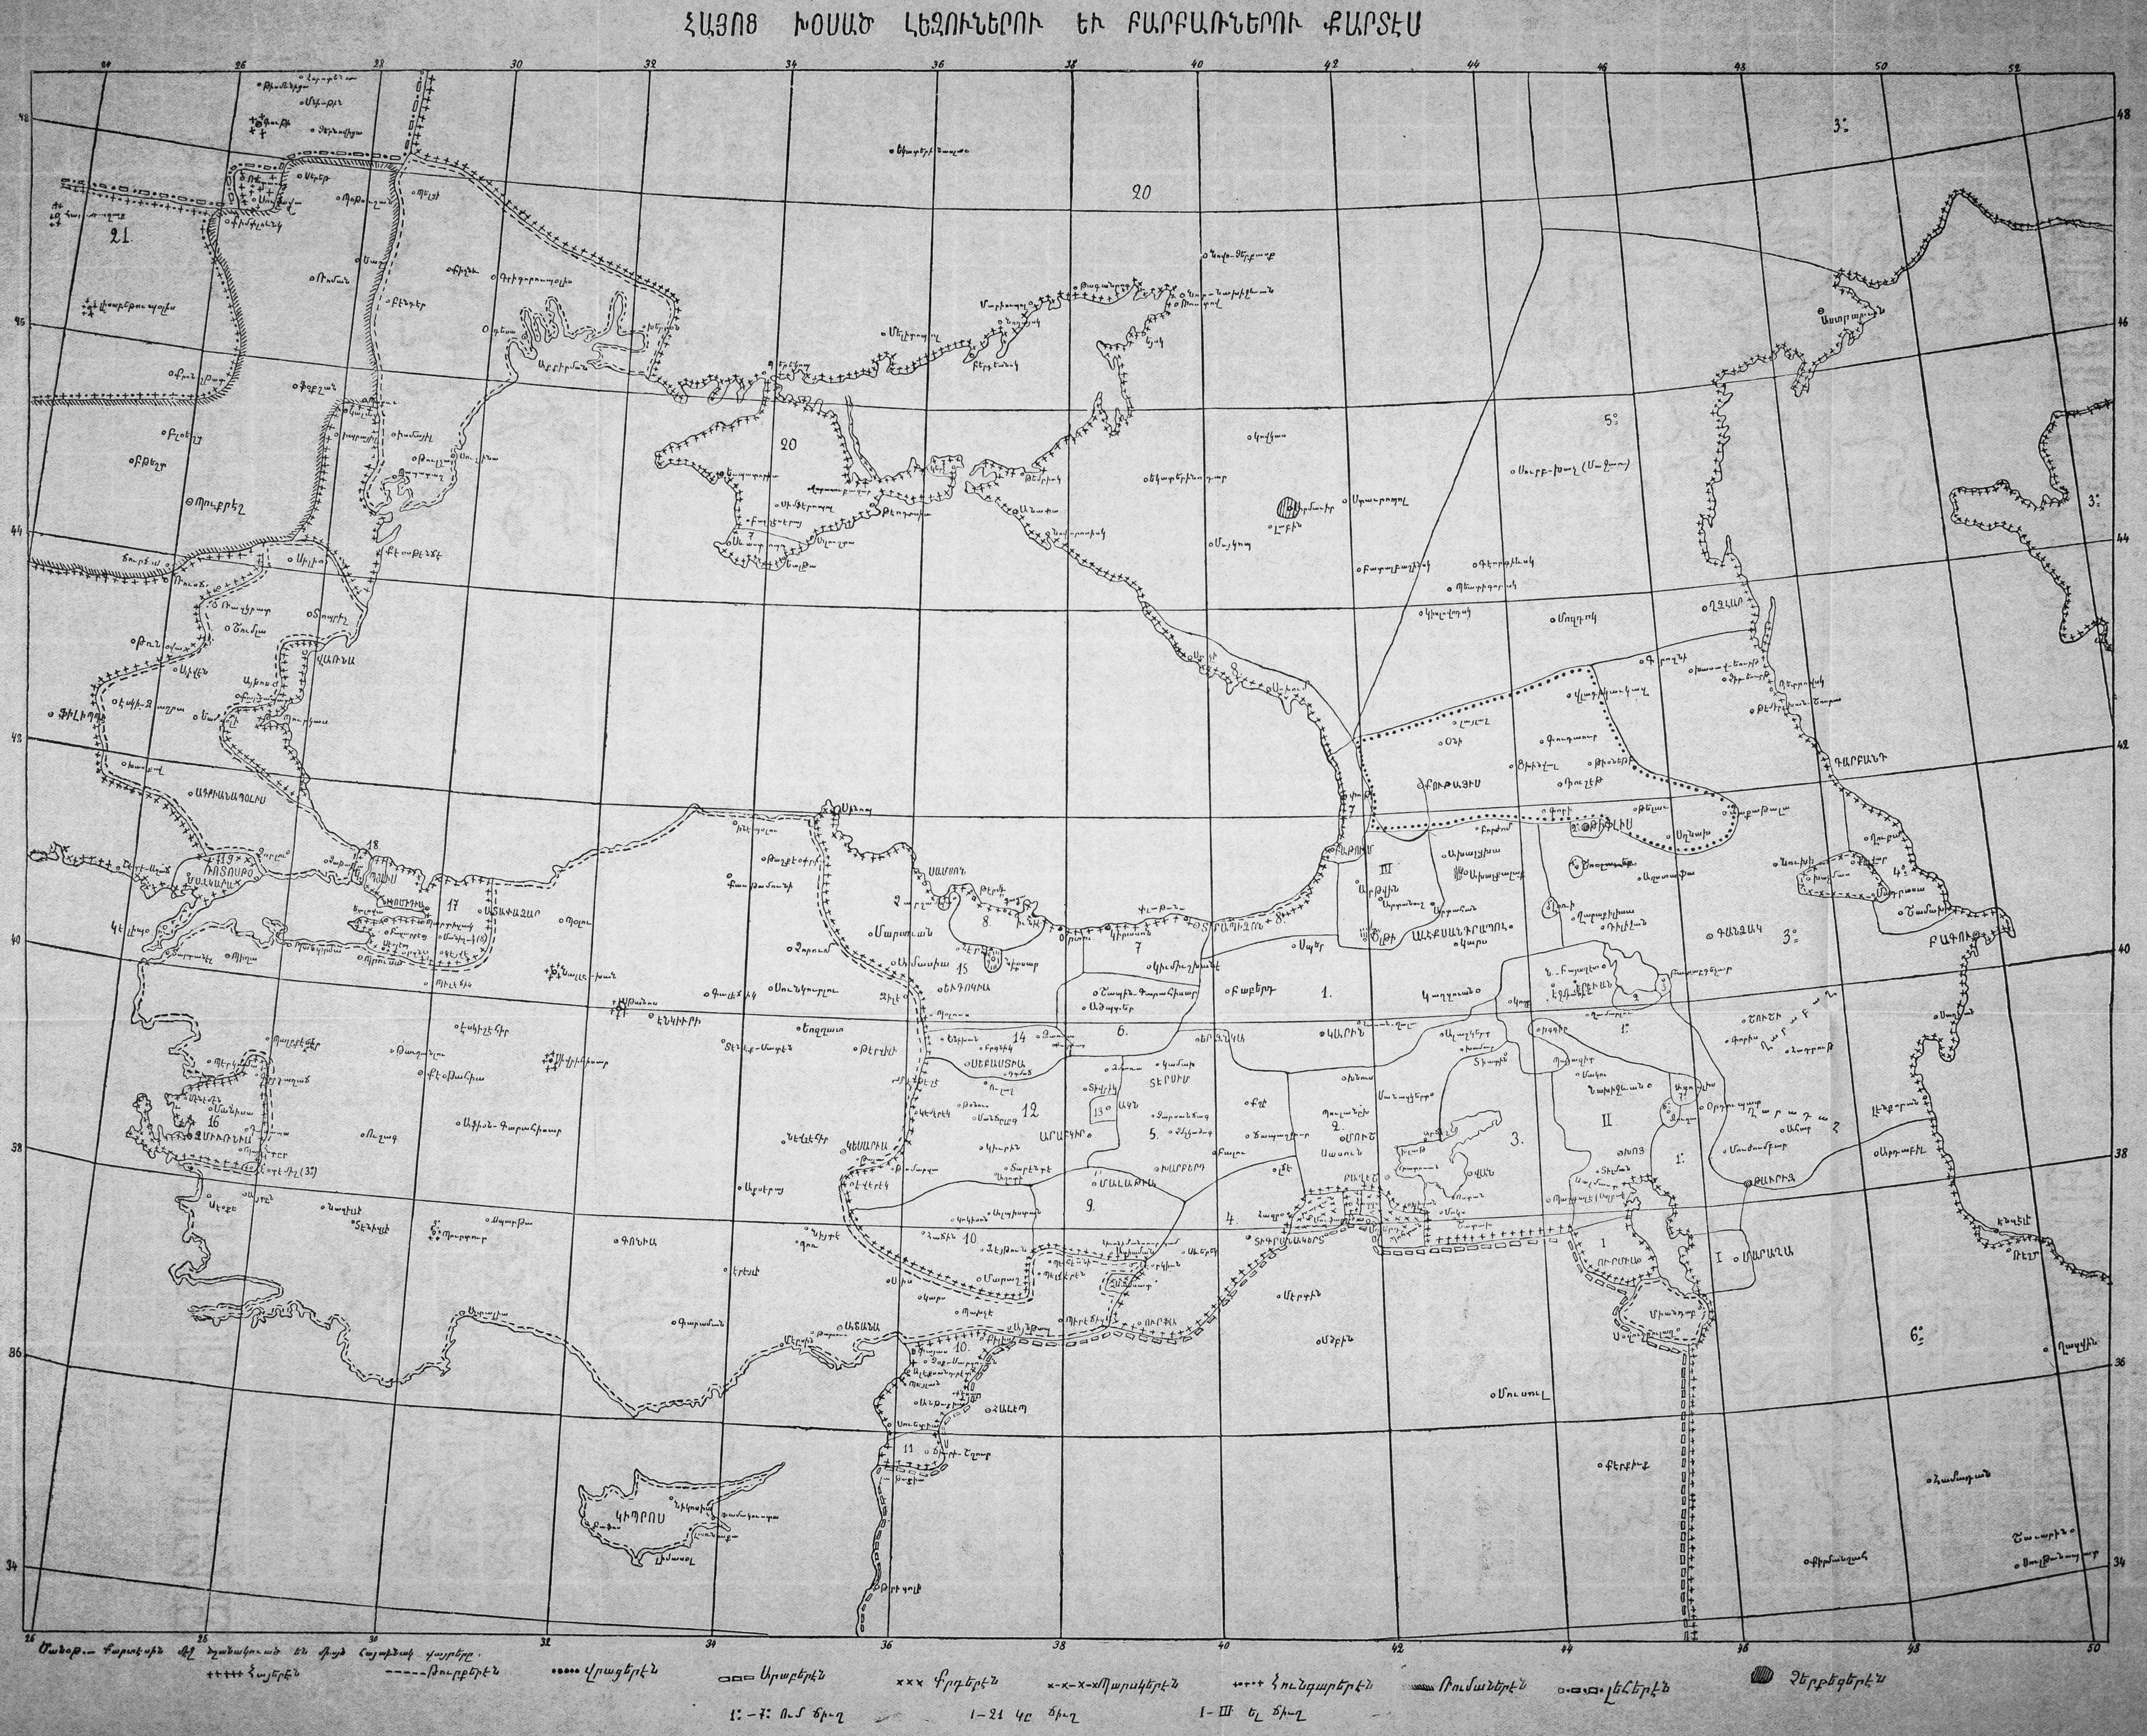
\includegraphics{images/map1911.png}
	}
\end{figure}




In the original 1909 French monograph, Adjarian provided a similar map. It   is displayed in Figure \ref{map:Adjarian1909}. The names are all in Armenian. 

\begin{figure}[H]
	\caption{Map from Adjarian 1909}
	\label{map:Adjarian1909}
	\resizebox{\textwidth}{!}{%
		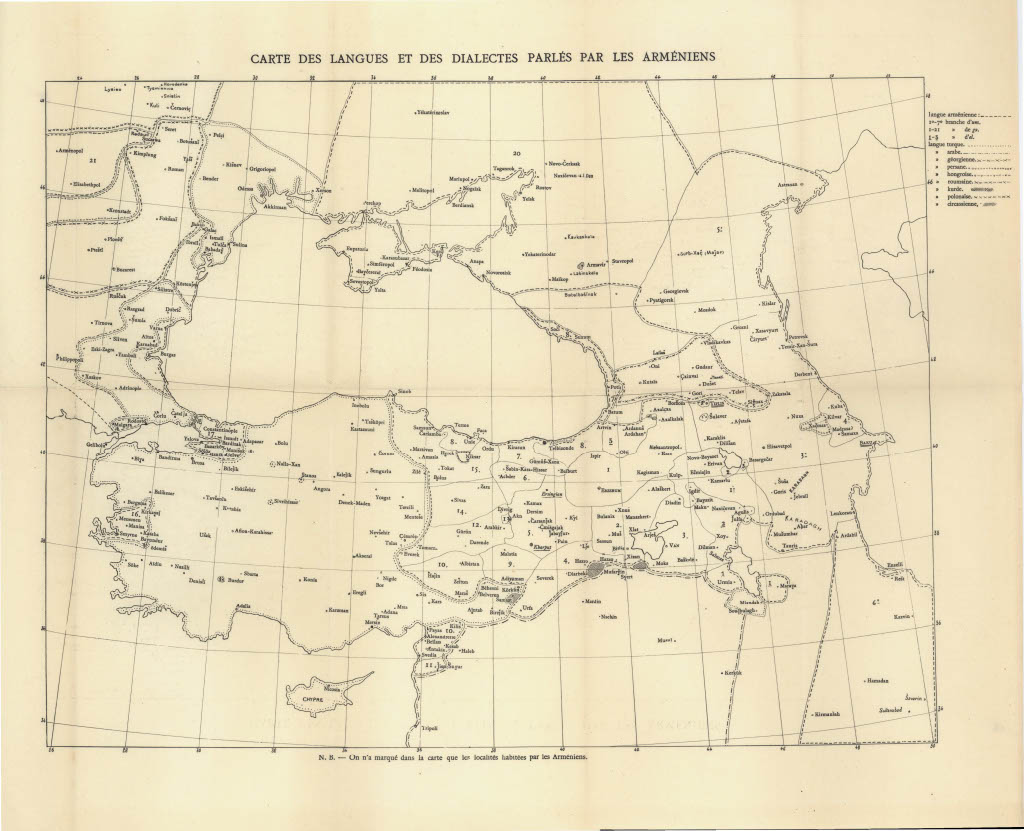
\includegraphics{images/map1909.jpg}
	}
\end{figure}

On Wikimedia, there is a modified form of the 1909 map that includes colorcoding.\footnote{\url{https://commons.wikimedia.org/wiki/File:Armenian_dialects,_Adjarian_1909.png}} It   is displayed in Figure \ref{map:Adjarian1909color}. The names are all in a romanized form; they don't however match the names that we used in our translation. 



\begin{figure}[H]
	\caption{Adapted map from Adjarian 1909 (from Wikimedia)}
	\label{map:Adjarian1909color}
	\resizebox{\textwidth}{!}{%
		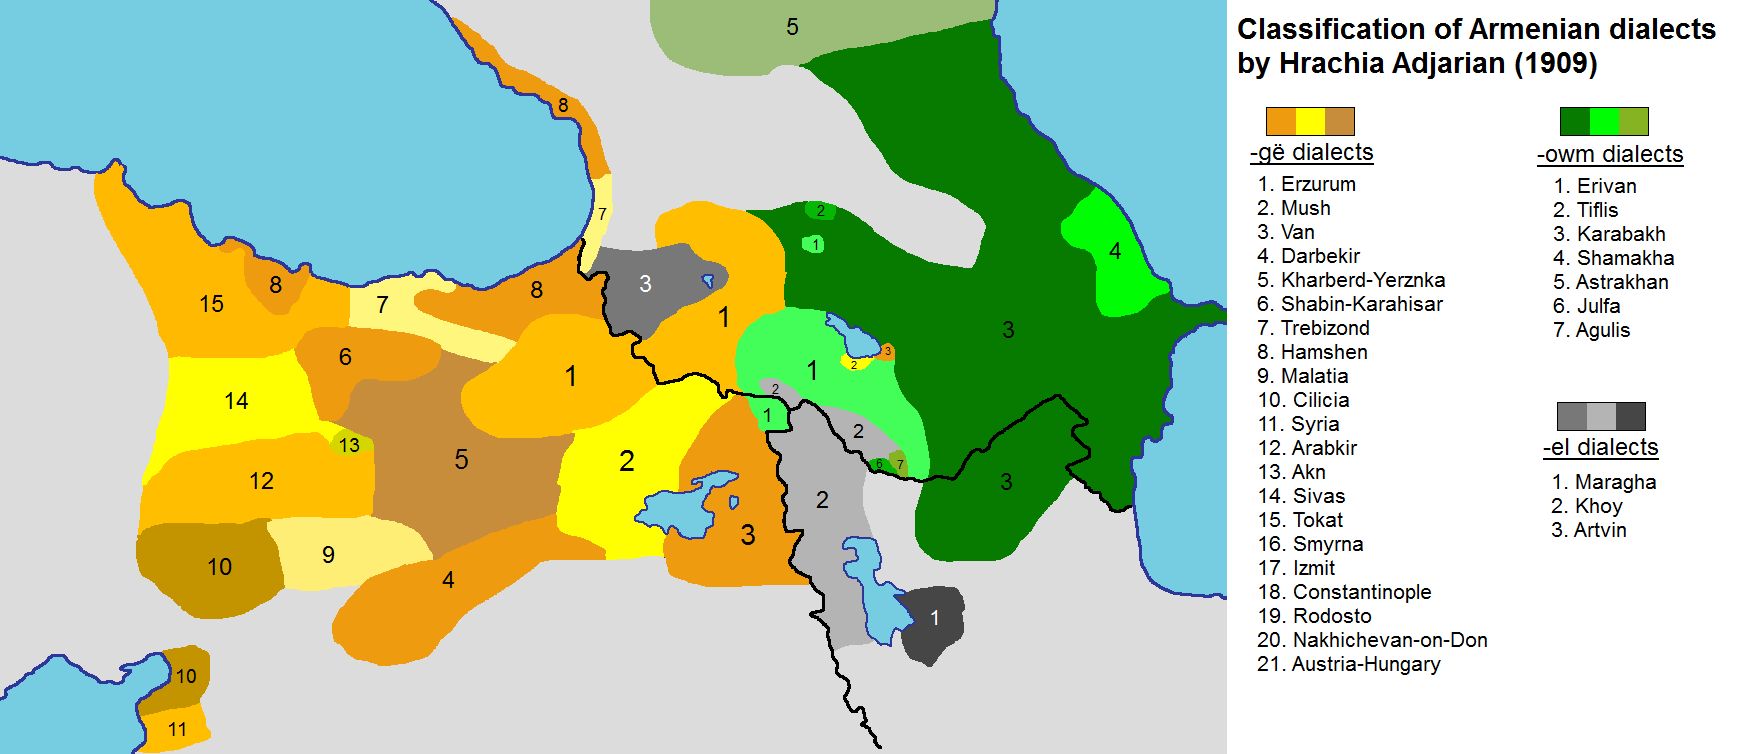
\includegraphics{images/map1909color.png}
	}
\end{figure}

 \section{Phonology of Armenian and our phonological transcription}\label{sec:HossepIntro:phonotransc}

This section explains the phonological transcriptions that I used in the translation. I explain my transcription system used for the modern standard varieties (\S\ref{sec:HossepIntro:phonotransc:modern}), Classical Armenian (\S\ref{sec:HossepIntro:phonotransc:CA}),  and non-standard dialects (\S\ref{sec:HossepIntro:phonotransc:adj}). In brief, I transcribe words in IPA based on their attested pronounciation (SEA/SWA)  or their most likely pronunciation (CA). For the non-standard dialects, Adjarian developed his own dialectological notation, for which I provide IPA approximations. 
\subsection{Phonology of Modern Standard Armenian}\label{sec:HossepIntro:phonotransc:modern}

Modern SEA and SEA are relatively well-studied in terms of their basic phonemic inventory and phonological transcriptions. I discuss nuances of transcribing SEA/SWA consonants (\S\ref{sec:HossepIntro:phonotransc:modern:cons}), vowels (\S\ref{sec:HossepIntro:phonotransc:modern:vowe}),  and stress (\S\ref{sec:HossepIntro:phonotransc:modern:stress}). 
\subsubsection{Consonant inventory}\label{sec:HossepIntro:phonotransc:modern:cons}
Table \ref{fig:HossepIntro:consSEA} provides the consonant inventories for SEA and SWA. Parantheses mark consonantal phonemes that are present in SEA but not SWA. 

\begin{table}[H]
	\caption{Consonant inventory of SEA and SWA}\label{fig:HossepIntro:consSEA}
	\resizebox{\textwidth}{!}{%
			\begin{tabular}{| l| lllllllll| }
			\hline 	& Bilabial & Labiodental & Dental & Alveolar & Postalveolar & Palatal & Velar & Uvular & Glottal \\
 
			\hline 	Stop & (p) pʰ b & & (t) tʰ d & & & & (k) kʰ ɡ & & \\
		Affricate & & & t͡s (t͡sʰ) d͡z & & t͡ʃ (t͡ʃʰ) d͡ʒ & & & & \\
		Nasal & m & & & n & & & & & \\
		Trill & & & & (r) & & & & & \\
		Tap & & & & ɾ & & & & & \\
		Fricative & & f v & & s z & ʃ ʒ & & & χ ʁ & h \\
		Approximant & & & & & & j & & & \\
		\hline 
	\end{tabular}
}
\end{table}

Phonologically, SEA has a three-way larnygeal contrast or voicing contrast among stops and affricates: voiced, voiceless unaspirated, and voiceless aspirated. Classical Armenian (CA) is argued to have had a similar three-way contrast as well. In contrast, SWA has a simpler two-way contrast: phonologically voiced and phonologically voiceless (Table \ref{tab:intro:ea wa differences: phono}). Conventionally, the SWA stops and affricates are treated as being voiced vs. voiceless aspirated.

\begin{table}[H]
	\caption{Three-way laryngeal contrast in SEA but not SWA}
	\label{tab:intro:ea wa differences: phono}
	\centering
	\begin{tabular}{|l|llll| lll| }
		\hline 	& CA & SEA & &  &SWA & & 
		\\
		/p/ & \textbf{p}ɑɾ& \textbf{p}ɑɾ & `dance' & \armenian{պար} & & & 
		\\
		/pʰ/ & \textbf{pʰ}ɑk & \textbf{pʰ}ɑk & `closed' &\armenian{փակ}& \textbf{pʰ}ɑk & `closed' & \armenian{փակ}
		\\
		/b/ & \textbf{b}ɑd & \textbf{b}ɑd & `duck' & \armenian{բադ} & \textbf{b}ɑɾ & `dance'& \armenian{պար} \\ \hline
	\end{tabular}
\end{table}

However, the phonetic manifestation of the SWA voicing contrast is subject to geographical variation due to language contact \citep{kellyKeshishian-2021-VoicingWesternArmenian,Tahtadjian-2021-PhoneticInterferenceProductionStopsWesternArmenianBilingual}. For example, the SWA-speaking community in Turkey has a voiced vs. voiceless aspirate distinction for stops and affricates: D vs. Tʰ, and D͡Z vs. T͡Sʰ. In contrast, the SWA-speaking community in Lebanon instead has a voiced vs. voiceless unaspirated distinction for stops and affricates : D vs. T, and D͡Z vs. T͡S. For this monograph, because Adjarian's socio-geographic subdialect of SWA had a traditional D-Tʰ distinction, I transcribe the SWA forms with a traditional D-Tʰ distinction. 

The change from a three-way contrast in CA to a two-way contrast in SWA is a major topic in the diachronic phonology of Armenian. Throughout this translation, Adjarian spends time in describing the consonantal changes for the various non-standard dialects. 


What follows  are minor comments on the  phonology or phonetics of the consonant inventory, based largely on recent survey-level phonetic work on SEA and SWA \citep{Seyfarth-JIPAArmenian}. 


\begin{itemize}
	\item Minor comments on SEA and SWA consonant inventory 
	\begin{enumerate}
		\item The coronal stops usually have a dental articulation. 
		\item The dorsal fricatives /χ, ʁ/ are typically described as uvular, but they can have a velar pronunciation. 
		\item SEA has a phonemic trill and tap/flap distinction /r, ɾ/, while modern SWA only has a flap /ɾ/. However, more archaic registers have a phonemic trill that has been largely lost for most modern communities \citep{Tahtadjian-2020-WesterArmenianRhoticDifferentialPhoneticStudy}. Adjarian 1911 however says that SWA still has a trill in his time (Table \ref{tab:intro:othersound}).  Out of respect for Adjarian's ideolect, I thus transcribe SWA forms in this translation with a trill. 
		\item Both dialects   have an allophonic sound [ŋ]. This velar nasal is used when a nasal /n/ precedes a velar stop, i.e., there is velar place assimilation. For SEA and SWA, I transcribe the velar stop. For example, the word /menkʰ/ `we' <\armenian{մենք}> is pronounced [meŋkʰ] in SEA/SWA.  
		
	\end{enumerate}
\end{itemize}

\subsubsection{Vowel inventory}\label{sec:HossepIntro:phonotransc:modern:vowe}
Table \ref{fig:HossepIntro:SEAvowel inventory} provides the vowel inventories of SWA and SEA. Parantheses mark vowels that are present in SWA but not SEA. 

\begin{figure}[H]
	\centering
	\caption{Vowel inventory of SEA and SWA}
	\label{fig:HossepIntro:SEAvowel inventory}
	\begin{tikzpicture}[scale=2]
		\large
		\tikzset{
			vowel/.style={fill=white, anchor=mid, text depth=0ex, text height=1ex},
			dot/.style={circle,fill=black,minimum size=0.4ex,inner sep=0pt,outer sep=-1pt},
		}
		\coordinate (hf) at (0,2); % high front
		\coordinate (hb) at (2,2); % high back
		\coordinate (lf) at (1,0); % low front
		\coordinate (lb) at (2,0); % low back
		\def\V(#1,#2){barycentric cs:hf={(3-#1)*(2-#2)},hb={(3-#1)*#2},lf={#1*(2-#2)},lb={#1*#2}}
		
		% Draw the horizontal lines first.
		\draw (\V(0,0)) -- (\V(0,2));
		\draw (\V(1,0)) -- (\V(1,2));
		\draw (\V(2,0)) -- (\V(2,2));
		\draw (\V(3,0)) -- (\V(3,2));
		
		% Place all the unrounded-rounded pairs next, on top of the horizontal lines.
		\path (\V(0,0)) node[vowel, left] {i} node[dot] {};
		% \path (\V(0,1)) node[vowel, left] {ɨ} node[vowel, right] {ʉ} node[dot] {};
		\path (\V(0,2)) node[vowel, right] {u} node[dot] {};
		\path (\V(0.5,0.4)) node[vowel, right] {(ʏ)} node[dot] {};
		% \path (\V(0.5,1.6)) node[vowel, left] { } node[vowel, right] {ʊ} node[dot] {};
		\path (\V(1,0)) node[vowel, left] {e}   node[dot] {};
		%\path (\V(1,0)) node[vowel, left] {e} node[vowel, right] {ø} node[dot] {};
		% \path (\V(1,1)) node[vowel, left] {ɘ} node[vowel, right] {ɵ} node[dot] {};
		\path (\V(1,2)) node[vowel, right] {o} node[dot] {};
	%	\path (\V(2,0))   node[vowel, right] {œ} node[dot] {};
		% \path (\V(2,0)) node[vowel, left] {ɛ} node[vowel, right] {œ} node[dot] {};
		% \path (\V(2,1)) node[vowel, left] {ɜ} node[vowel, right] {ɞ} node[dot] {};
		% \path (\V(2,2)) node[vowel, left] {ʌ} node[vowel, right] {ɔ} node[dot] {};
		% \path (\V(2.5,0)) node[vowel, left] {æ} node[vowel, right] { } node[ ] {};
		% \path (\V(3,0)) node[vowel, left] {a} node[vowel, right] {ɶ} node[dot] {};
		\path (\V(3,2)) node[vowel, left] {ɑ} node[dot] {};
		
		% Draw the vertical lines.
		\draw (\V(0,0)) -- (\V(3,0));
		\draw (\V(0,1)) -- (\V(3,1));
		\draw (\V(0,2)) -- (\V(3,2));
		
		% Place the unpaired symbols last, on top of the vertical lines.
		\path (\V(1.5,1)) node[vowel] {ə};
		% \path (\V(2.5,1)) node[vowel] {ɐ};
	\end{tikzpicture}
\end{figure}


In general, the SWA sound /ʏ/ corresponds to an SEA /ju/ sequence. Some SWA loanwords have a vowel /œ/, but this vowel is quite marginal and found in only a handful of loanwords. 

The midvowels are sometimes transcribed as lax /ɛ, ɔ/ in the phonological literature \citep{Vaux-1998-ArmenianPhono}. But more recent phonetic work suggests that these vowels don't have an open-mid articulatory/acoustic target, but are instead close-mid /e, o/ \citep{Toparlak-2019-MAArmenianPhonetics,Seyfarth-JIPAArmenian}.\footnote{For my own SWA ears, I cannot perceive the difference between [e, ɛ], suggesting that Armenian has a generic articulatory target for midvowels.}
	
\subsubsection{Stress}\label{sec:HossepIntro:phonotransc:modern:stress}




SWA and SEA generally have final stress. If the last syllable has a non-schwa vowel, that vowel has stress (\ref{sent:HossepIntro:CA:stress:final}). But if the last syllable has a schwa, while the penultimate syllable has a non-schwa, then the penultimate syllable gets stress (\ref{sent:HossepIntro:CA:stress:penult}). 

\begin{exe}
	\ex SEA \label{sent:HossepIntro:CA:stress}
	\begin{xlist}
		\ex \gll kɑp\'ik \\
		monkey \\
		\trans `monkey' \label{sent:HossepIntro:CA:stress:final}\\
		\armenian{կապիկ}
		\ex \gll kɑp\'ik-ə \\
		monkey-{\defgloss} \\
		\trans `the monkey' \label{sent:HossepIntro:CA:stress:penult} \\
		\armenian{կապիկը}
		
	\end{xlist}
\end{exe}

There are some morphological exceptions to final stress. In early SWA, the suffix sequence /-e-i/ ({\thgloss}-{\pst}) in the imperfective past gets regular final stress. But in  most modern SWA communities, this suffix sequence gets penultiamte stress. I seems that in Adjarian's time, this change didn't take place yet. So I transcribe this SWA suffix sequence with final stress in this monograph. 

\subsection{Classical Armenian pronunciations and phonology}\label{sec:HossepIntro:phonotransc:CA}

Classical Armenian or CA is the oldest attested variety of Armenian. The earliest written records are from the fifth century. It is a dead language, so we don't know its exact pronunciation, but we do have suggestive evidence (\S\ref{sec:HossepIntro:phonotransc:CA:approx}).  I set up my IPA transcription for  Classical Armenian for its monophthongal vowels (\S\ref{sec:HossepIntro:phonotransc:CA:mono}), diphthongal vowels (\S\ref{sec:HossepIntro:phonotransc:Classical:Diphthong}), consonants (\S\ref{sec:HossepIntro:phonotransc:CA:cons}), epenthetic schwas in consonant clusters (\S\ref{sec:HossepIntro:phonotransc:CA:schwa}), and stress (\S\ref{sec:HossepIntro:phonotransc:CA:stress}). 

 

\subsubsection{Approximating   the phonology of Classical Armenian}\label{sec:HossepIntro:phonotransc:CA:approx}
Classical Armenian (CA) is an ancient dead language. We have no access to speakers, recordings, or phonetic analyses of CA. Thus, we will never know exactly what CA sounded like. Instead, we can approximate a probable CA phonology using the following pieces of information:
\begin{enumerate}
	\item orthography and transliteration conventions
		\item traditional pronunciation
\item post-Classical phonological changes
\end{enumerate}

To clarify the above points, Classical Armenian is written using the Armenian script. The script was invented in order to write Classical Armenian. It is thus likely that the orthography is close to the pronunciation of Classical Armenian. The orthography is traditionally transliterated using the Hübschmann-Meillet-Benveniste transliteration system (HMB). Transliteration schemes can be found online, such as Wiktionary.\footnote{\url{https://en.wiktionary.org/wiki/Wiktionary:Armenian_transliteration}} The transliteration is not a phonological nor phonetic transcription, but it does help us determine approximate IPA symbols for CA. 

As for pronunciation, although CA is a dead language, there is a conventional system for how to read CA texts. This system is called `traditional pronunciation'. It was formulated sometime after the first written record of CA. An approximate date for this formulation is between the 8th and 12th centuries (\citealt[24]{Godel-1975-IntroClassicalArmenian}; \citealt[1039]{Macak-2017-PhonoClassicalArmenian}). The formulated conventions indicate a mix of phonological patterns that were attested in CA or that developed later in the post-Classical period.

For this book, I transcribe all CA forms using IPA. I do not use transliteration. The rationale is that transliteration systems by themselves do not unambiguously reflect the most likely phonological form of CA words. In order to understand the various sound changes from CA to the modern dialects, it is more practical to transcribe both CA and modern Armenian in their phonological form, i.e, by using IPA symbols.\footnote{This concern is especially important for cases where the transliteration is utterly confusing from a phonological point of view. For example, the affricate series <\armenian{ձ, ծ, ց, ջ, ճ, չ}> is conventionally transliterated as <j, c, cʿ,  ǰ, č, čʿ> but its most likely pronunciation is /d͡z,   t͡s,    t͡sʰ,   d͡ʒ,   t͡ʃ,   t͡ʃʰ/.  The CA low vowel <\armenian{ա}> was likely a low back /ɑ/, and developed to SEA /ɑ/, and to dialectal /ɑ, æ/. The CA transliteration is <a>, and such a symbol is a front vowel /a/ in the IPA. The rhotic series <\armenian{ր, ռ}> developed to SEA /ɾ, r/, and were likely /ɾ, r/ in CA. But the transliteration as <r, ṙ> would confuse the non-trill and trilled symbols.}



\subsubsection{Monophthong vowel inventory}\label{sec:HossepIntro:phonotransc:CA:mono}

Classical Armenian has seven basic monopthong vowels. These vowels are listed in Table \ref{tab:HossepIntr:classicalVowel}. I provide the native orthographic form, the HBM transliteration, and an approximate IPA symbol. 



\begin{table}[H]
	\centering
	\caption{Monophthong vowels of Classical Armenian}
	\label{tab:HossepIntr:classicalVowel}
	\begin{tabular}{|l|lllllll|}
		\hline 
		Orthography & \armenian{ա} & \armenian{ե} & \armenian{է} & \armenian{ը}& \armenian{ի} & \armenian{ո} & \armenian{ու}\\
		HMB transliteration & a & e & ē & ə & i & o & u \\
		IPA transcription & ɑ & e & ē & ə & i & o & u 
		\\ \hline
	\end{tabular}
\end{table}



For the IPA transcription of Classical Armenian vowels, I adapt conventional transcriptions from the traditional pronunciation and from the modern standard dialects in the following way. 


For the grapheme <\armenian{ա}>, the modern standard dialects use a low back unrounded vowel /ɑ/. We don't know exactly what the ancient language used. For simplicity and illustration, we assume the Classical low vowel was likewise back. This seems to be an implicit assumption by Adjarian as well, because he later uses a different symbol <\armenian{ա}̈> to mark the low front vowel /æ/. 

For the front midvowel pair <\armenian{ե, է}>, we don't know the exact phonetic difference in Classical Armenian. The two graphemes are often transliterated as <e> vs. <ē>, and they are argued to have a phonological contrast in terms of tenseness \citep[14]{Thomson-1989-IntroClassicalArmenian} or length \citep[6]{Godel-1975-IntroClassicalArmenian}. Some  possible transcriptions are /ɛ/ vs. /e/,  or /e/ vs. /eː/. 

Within the IPA, the macron   ̄  indicates tone but philology often uses a macron to indicate long vowels and heavy syllables. This philological tradition is likely the reason why the HBM transliteration uses /ē/. For this translation,   I transcribe the two vowels as /e/ vs. /ē/, in keeping with the transliteration. The reason is because we ultimately don't know the actual phonological or phonetic  difference between the two vowels. All we need to know is that one vowel (the tense or long \armenian{է}) is considered the `marked' form. 


For the midvowels <\armenian{ե, ո}>, the modern standard dialects can range between using low-mid /ɛ,ɔ/ and high-mid /e,o/. Such variation is free variation in my experience. For simplicity, I transcribe them high-mid /e,o/ instead of low-mid /ɛ,ɔ/, contra \citet[1039]{Macak-2017-PhonoClassicalArmenian}. 

The segments <\armenian{ը, ի, ու}> are transliterated and traditioally pronounced as /ə, i, u/. 

\subsubsection{Diphthong vowel inventory}\label{sec:HossepIntro:phonotransc:Classical:Diphthong}
In addition to monophthongal vowels, Classical Armenian had nine diphthongs (Table \ref{tab:HossepIntr:classicalDiphthong}). 


\begin{table}[H]
	\centering
	\caption{Diphthong vowels of Classical Armenian}
	\label{tab:HossepIntr:classicalDiphthong}
	\begin{tabular}{|l|lllllllll|}
		\hline 
		Orthography & \armenian{այ} & \armenian{աւ} & \armenian{եա} & \armenian{եւ} & \armenian{եայ}& \armenian{եաւ}& \armenian{իւ} & \armenian{ոյ} & \armenian{ուա}\\
		HMB transliteration & ay & aw & ea & ew & eay& eaw& iw & oy & ua\\
		IPA transcription & ɑi̯ & ɑu̯ &e̯ɑ & eu̯ & e̯ɑi̯& e̯ɑu̯ & iu̯ & oi̯ & u̯ɑ
		\\ \hline
	\end{tabular}
\end{table}

Orthographically, Classical Armeinan diphthongs are made up of a) a vowel plus a glide symbol like <\armenian{այ}> <ay>, b) two vowels like <\armenian{եա}> <ea>, or c) a combination of vowels and glides like <\armenian{եաւ}> <eaw>. 

These orthographic sequences like <\armenian{այ}> <ay> were pronounced and phonologically treated as diphthongs like [ɑi̯] and not as vowel-glide sequences like [ɑj]. The evidence is the following. Philological and dialectological work uses the term `diphthong' (Armenian: [jeɾkbɑɾbɑr] <\armenian{երկբարբառ}>, literally `two-sounds' in Classical Armenian). In the modern standard languages, orthographic vowel-glide sequences like <ay> are pronouned as vowel-glides sequences /ɑj/, and philologists like Adjarian explicitly state that the standard dialects lack diphthongs (\S\ref{sec:AdjarianIntro:difference:soundChange:DiphthongLoss}). 

As for their IPA values, it is difficult to give a meaningful transcription for Classica diphthongs. I follow \citet{Macak-2017-PhonoClassicalArmenian} in placing an inverted breve under the less prominent member of the diphthong (= what would correspond to a high vowel). I note the following minor notatonal differences between my transcription and Macak. 

\begin{itemize}
		\item For <\armenian{եա}> <ea>, \citet[1041,1043]{Macak-2017-PhonoClassicalArmenian} suggests /i̯ɑ/ but I opted for /e̯ɑ/ because it's more faithful to the orthography. 
		\item For <\armenian{իւ}> <iw>, \citet[1041,1043]{Macak-2017-PhonoClassicalArmenian} notes that this cluster can be pronounced as either /iu̯/ or /i̯u/ depending on phonological position. I opt for a uniform /iu̯/ because Adjarian does not notice such differences.
		\item For <\armenian{ոյ}>, the traditional pronunciation is /ui̯/ \citep[1039]{Macak-2017-PhonoClassicalArmenian}. But, the orthography suggests that this digraph was pronounced as /oi̯/. 
\end{itemize}

For <\armenian{եայ}>, I could not find a pre-established convention so I use /e̯ɑi̯/. 
	
There is some ambiguity when an orthographic diphthong is pre-vocalic like <\armenian{այա}> or <\armenian{աւա}>. The HMB transliteration is just <aya, awa>. Phonologically, I suspect the offlgide would have acted as a consonantal onset /ɑjɑ, ɑwɑ/ and not as a sequence of vowels /ɑi̯ɑ, ɑu̯ɑ/. I thus transcribe such pre-vocalic diphthongs as vowel-glide sequences. However, note that Adjarian seems to phonologically treat these pre-vocalic forms as still phonologically diphthongs instead of vowel-glide sequences (\ref{page:64}). 




There are other attested orthographic vowel-vowel sequences such as <\armenian{ուէ}> <uē> in <\armenian{աղուէս}> `fox' and <\armenian{ուի}> <ui> in <\armenian{թուիլ}> `to appear'. For these, the HMB transliteration would be <aɬuēs> and <tʿuil>. Their modern SEA pronunciations would use a /v/ in place of the <\armenian{ու}>: /ɑʁves, tʰəvil/. It's unclear if historically such orthographic sequences were some type of diphthong too: /ɑɬu̯es, tʰu̯il/. But it is seems that the convention is to treat the digraph <\armenian{ու}> as a non-alternating /u/ \citep[15]{Thomson-1989-IntroClassicalArmenian}, and allow it to be part of vowel hiatus \citep[17]{Thomson-1989-IntroClassicalArmenian}. To be safe, I treat such sequences then as vowel hiatus as well: /ɑɬu.es, tʰu.il/.\footnote{It has been suggested that the initial /u/ in vowel hiatus is rendered as [əw] \citep[13]{Kim-2021-phoneticsPhonologyOldArmenianWV}. Thus CA /ɑɬues/ `fox' could have been pronounced as [ɑɬəwes].  }

Note that Classical grapheme sequence <\armenian{աւ}> /ɑu̯/ became SEA /o/, and this change encouraged the use of a new letter <\armenian{օ}> in its place. Adjarian often uses the letter <\armenian{օ}> to refer the ancient diphthong. When he does use the letter <\armenian{օ}> in these contexts (such as <\armenian{մօր}> `mother.{\gen}), I use the transliteration <ō> and the Classical pronunciation /ɑu̯/: <mōr>, /mɑu̯ɾ/. I usually opt to use an alternative CA spelling with <\armenian{աւ}>: <\armenian{մաւր}> <mawɾ> /mɑu̯ɾ/. I do this so that it's clearer what were the actual sound changes from Classical Armenian to the modern dialects. 


\subsubsection{Consonant inventory}\label{sec:HossepIntro:phonotransc:CA:cons}



Classical Armenian had 30 consonants (Table \ref{tab:HossepIntr:classicalConsonant}). 

\begin{table}[H]
	\centering
	\caption{Consonants of Classical Armenian}
	\label{tab:HossepIntr:classicalConsonant}
	\begin{tabular}{|l|lllllllll|}
		\hline 
		Orthography & \armenian{բ} &\armenian{պ}& \armenian{փ} &\armenian{դ}& \armenian{տ} &\armenian{թ}& \armenian{գ}& \armenian{կ}& \armenian{ք} \\
		HMB transliteration & b &p& pʿ &d& t &tʿ& g& k& kʿ \\
		IPA transcription & b &p& pʰ &d& t &tʰ& ɡ& k& kʰ \\
		\hline 
		Orthography &\armenian{ձ}& \armenian{ծ}& \armenian{ց} &\armenian{ջ}& \armenian{ճ}& \armenian{չ} & & & \\
		HMB transliteration &j &c &cʿ& ǰ &č &čʿ & & & \\
		IPA transcription & d͡z & t͡s & t͡sʰ & d͡ʒ & t͡ʃ & t͡ʃʰ & & & \\
		\hline 
		Orthography & \armenian{վ} & \armenian{ս}& \armenian{զ}& \armenian{շ}& \armenian{ժ}& \armenian{խ} & \armenian{հ} & & \\
		HMB transliteration & v & s& z& š& ž& x & h & & \\
		IPA transcription& v & s& z& ʃ& ʒ& χ & h & & 
		\\ 
		\hline
		Orthography & \armenian{մ} & \armenian{ն} & \armenian{ր}& \armenian{ռ}& \armenian{լ}& \armenian{ղ} & \armenian{ւ} & \armenian{յ} & \\
		HMB transliteration & m & n & r & ṙ&l & ł & w & y & \\
		IPA transcription & m & n & ɾ & r& l & ł & w & j& 
		\\ \hline 
	\end{tabular}
\end{table}

For stops and affricates, Classical Armenian had a three-way laryngeal contrast. These contrast is conventionally treated as between voiced, voiceless unaspirated, and voiceless aspirated /b, p, pʰ/. 

For the fricatives, these are generally uncontroversial. 		 For the back fricative <\armenian{խ}>, the modern standard dialects show free variation between a velar /x/ vs. uvular /χ/ articulation. The uvular transcription is however more typical. I use the uvular form as the default transcription for Classical Armenian. 

For the nasals, the modern standard dialects have an allophonic velar nasal [ŋ] that's used when a coronal nasal /n/ precedes a velar stop. The Armenian orthography does not mark this in any variety, including Classical Armenian. It is unknown if Classical Armenian likewise had nasal place assimilation before velar stops, but it is likely. To be safe, I don't use a velar nasal [ŋ] for Classical Armenian. 

For the rhotics <\armenian{ր,ռ}> or <r, ṙ>, they are pronounced as a flap vs. trill in the modern SEA /ɾ, r/. It's unclear if the <\armenian{ր}> was a flap /ɾ/ or an approximant /ɹ/ in the Classical language \citep[1040]{Macak-2017-PhonoClassicalArmenian}. I opt for a flap /ɾ/. Adjarian himself does not comment on the pronunciation of this rhotic. 


For the liquids, the symbol <\armenian{լ}> <l> is pronounced as a simple lateral /l/ in the traditional pronunciation and the modern standard dialects. The symbol <\armenian{ղ}> <ɬ> is pronounced as a voiced uvular fricative /ʁ/ in the modern standard dialects, while it is generally treated as a dark or velar lateral /ɬ/ in Classical Armenian (\S\ref{sec:AdjarianIntro:difference:soundChange:VelarGlide}, \citealt[ch2]{Macak-2016-StudiesClassicalModernArmenianPhono}).

For the sonorants <\armenian{յ, ւ}>, these are traditionally transliterated as <y,w>. These sounds are the glides /j,w/. However, it is difficult to know when such a letter was pronounced as a glide vs. part of a diphthong (\S\ref{sec:HossepIntro:phonotransc:Classical:Diphthong}). 

\subsubsection{Schwa epenthesis}\label{sec:HossepIntro:phonotransc:CA:schwa}


Classical Armenian has a schwa symbol <\armenian{ը}> /ə/. This vowel is written in some words like /əst/ <\armenian{ըստ}> <əst> `for'. However, it is likely that the sound /ə/ was pronounced in many words but was unwritten in the orthography. 

In the modern standard dialects, the orthography has long clusters of consonants (Table \ref{tab:HossepIntro:schwaEpen}). These clusters are broken up by schwas in pronunciation. A conventional analysis is to treat these schwas as epenthetic \citep{Vaux-1998-ArmenianPhono}. The patterns for epenthesis are complicated but rule-governed \citep[cf.][]{Dolatian-prep-Schwa}. It is likely that these epenthetic schwas were present likewise in Classical Armenian. 



\begin{table}[H]
	\caption{Schwa epenthesis in Classical Armenian and the standard dialects} \label{tab:HossepIntro:schwaEpen}
	\centering 
	\begin{tabular}{|l| lll| l| }
		\hline `fire'	& CA & SEA & SWA & \\
		<krak> & k\textbf{ə}ɾɑk &k\textbf{ə}ɾɑk &ɡ\textbf{ə}ɾɑɡ & \armenian{կրակ}
		\\\hline 
	\end{tabular}
\end{table}

There are various reasons to assume that Classical Armenian had the same unwritten schwa epenthesis rules as the modern standard dialects. In the traditional pronunciation, the convention is to pronounce unwritten schwas in almost exactly the same places as their modern forms (\citealt[16]{Godel-1975-IntroClassicalArmenian}; \citealt[116]{Thomson-1989-IntroClassicalArmenian}; \citealt[1043]{Macak-2017-PhonoClassicalArmenian}). Diachronically, some of these unwritten schwas are reflexes of Proto-Indo-European full vowels, that got reduced in Proto-Armenian \citep[26]{Vaux-1998-ArmenianPhono}. There is no synchronic evidence of an unreduced vowel in the underlying form for these unwritten epenthetic schwas.

There have been a few attempts at formalizing the rules for pronouncing these unwritten schwas for Classical Armenian \citep{Hammalian-1984-PhonoOldArmenian,Schwink-1994-ArmenianSchwaLexicalized,Pierce-2007-SchwaClassicalArmenian}. \citet{Pierce-2007-SchwaClassicalArmenian} has noted that as a spelling-pronunciation rule, essentially the same schwa epenthesis rules are active for Classical Armenian and for Modern Armenian.

Because of the above facts, I transcribe Classical Armenian with essentially the same epenthetic schwas that the modern standard dialects use. There are some situations where the traditional prononuciation of Classical Armenian sometimes uses an epenthetic schwa while the standard dialects don't. Two such situations are the suffix /-kʰ/ and the prefix /z-/. 

The suffix /-kʰ/ <\armenian{ք}> is a nominalizer in SEA and SWA. In the modern language, it does not use schwa epenthesis after stops or two consonants: [pɑɾt-kʰ] `debt' <\armenian{պարտք}>. But there are ambiguous and contradictory reports that the CA ancestor form (the plural suffix \textit{-kʰ}) does use schwa epenthesis in more contexts than SEA/SWA. For example, \citet[18-19]{Godel-1975-IntroClassicalArmenian}'s prose suggests schwa epenthesis applies after a CC cluster [pɑɾt-əkʰ] or after a stop/affricate. In contrast, \citet[120]{Thomson-1989-IntroClassicalArmenian}'s prose suggests no schwa epenthesis after a CC cluster [pɑɾt-kʰ]. Thomson suggests that schwa epenthesis applies only if the /-kʰ/ follows a velar stop. For these limited cases where schwa epentheiss is unclear, I transcribe the CA forms with a question mark: [pɑɾt-(ə?)kʰ]. 

The prefix /z-/ was an accusative prefix in Classical Armenian. When this prefix is before a consonant, a schwa is added before the prefix: /z-CV/$\rightarrow$[əz-CV] \citep[116]{Thomson-1989-IntroClassicalArmenian}. This prefix does not have a widely-used surviving reflex in SWA and SEA.


\subsubsection{Stress}\label{sec:HossepIntro:phonotransc:CA:stress}

 
In terms of stress, we don't have direct evidence from Classical sources. However, it is a convention to treat Classical Armenian as having the same basic stress patterns as the modern standard dialects (SEA and SWA), described in \S\ref{sec:HossepIntro:phonotransc:modern:stress}. 

Briefly, stress  is on the final non-schwa vowel of the word. in SEA an SWA. For Classical Armenian, the same stress rules are assumed to apply (\citealt[15]{Thomson-1989-IntroClassicalArmenian}; \citealt[1043-4]{Macak-2017-PhonoClassicalArmenian}). Evidence for the existence of final stress in pre-modern Armenian is discussed in \citet{DeLisi-2018-ArmenianProsodyDiachrony}.





\subsection{Adjarian's dialectological notation }\label{sec:HossepIntro:phonotransc:adj}


In the original monograph, Adjarian set up his own notation to capture the pronunciation of words from  non-standard dialects. He called his system a `scientific alphabet'  (\S\ref{sec:IntroAdjarian:scientificAlphabet}), and he adapted it from the Armenian script. I converted his notation to IPA, as explained in \S\ref{sec:HossepIntro:phonotransc:adj:ipa}. When re-transcribing his notation, I had to make decisions on matters that Adjarian kept implicit (\S\ref{sec:HossepIntro:phonotransc:adj:implicit}). I sometimes had to diverge from Adjarian's notation because of   typographic problems (\S\ref{sec:HossepIntro:phonotransc:adj:typograph}). I discovered that Adjarian had unfortunate inconsistencies in representing diphthongs (\S\ref{sec:HossepIntro:phonotransc:adjerror}). 


\subsubsection{IPA approximations}\label{sec:HossepIntro:phonotransc:adj:ipa}

In the original monograph, Adjarian transcribed what he perceived was the pronounciation of the non-standard dialects. He devised his own notation system based off of the Armenian alphabet, by adding additional diacritics or modifying the direction of letters. I call this his dialectological notation. 

In this translation, I retained his original dialectological transcriptions and supplied  an IPA approximation. Table \ref{tab:adjIPA}  lists all the dialectological symbols that he used, along with my IPA approximation and my  prosaic description. The PDF (and source LaTeX) of the translation can be searched for the occurrences of these symbols. Adjarian's prosaic description was  helpful in determining their phonetic values.  



\begin{center}
\begin{longtable}{|p{2.cm} p{2cm} p{7cm}|}

		\caption{Adjarian's  dialectological notation and my IPA approximations } \label{tab:adjIPA} \\ \hline
		\hline Adjarian's notation & IPA approximation & Description \\
		\hline 
		\multicolumn{3}{|l|}{Consonants}					\\ 
\armenian{բ}	& 	b 	& 	voiced bilabial stop	\\
		\armenian{բՙ}	& 	bʰ	& 	voiced aspirated bilabial stop	\\
		\armenian{դ}	& 	d 	& 	voiced coronal (dental) stop	\\
		\armenian{դՙ}	& 	dʰ	& 	voiced aspirated coronal (dental) stop	\\
		\armenian{ձ}	& 	d͡z 	& 	voiced coronal (dental) affricate	\\
		\armenian{ձՙ}	& 	d͡zʰ	& 	voiced aspirated coronal (dental) affricate	\\
		\armenian{ջ}	& 	d͡ʒ	& 	voiced postalveolar affricate	\\
		\armenian{ջՙ}	& 	d͡ʒʰ	& 	voiced aspirated postalveolar affricate	\\
		\armenian{ֆ}	& 	f	& 	voiceless labiodental fricative	\\
		\armenian{գ}	& 	ɡ 	& 	voiced velar stop	\\
		\armenian{գՙ}	& 	ɡʰ	& 	voiced aspirated velar stop	\\
		\armenian{գյ}	& 	ɡʲ	& 	palatalized voiced velar stop	\\
		\armenian{հՙ}	& 	ħ	& 	 voiceless pharyngeal fricative	\\
		\armenian{հ}	& 	h 	& 	voiceless glottal fricative	\\
		\armenian{հյ}	& 	hʲ	& 	palatalized voiceless glottal fricative	\\
		\armenian{՚, յ̵},   \armeniang{ֈ}	& 	ɦ	& 	voiced glottal fricative	\\
		\armenian{յ}	& 	j	& 	voiced palatal glide	\\
		\armenian{կ}	& 	k 	& 	voiceless unaspirated velar stop	\\
		\armenian{ք}	& 	kʰ	& 	voiceless aspirated velar stop	\\
		\armenian{քյ}	& 	kʰʲ	& 	palatalized voiceless aspirated velar stop	\\
		\armenian{կյ}	& 	kʲ	& 	palatalized voiceless unaspirated velar stop	\\
		\armenian{լ}	& 	l	& 	voiced lateral approximant	\\
		\armenian{լՙ}	& 	lʲ	& 	palatalized voiced lateral approximant	\\
		\armenian{մ}	& 	m 	& 	voiced bilabial nasal	\\
		\armenian{ն}	& 	n 	& 	voiced coronal (dental) nasal	\\
		\armenian{պ}	& 	p	& 	voiceless unaspirated bilabial stop	\\
		\armenian{փ}	& 	pʰ	& 	voiceless aspirated bilabial stop	\\
		\armenian{ղՙ}	& 	q	& 	voiceless uvular stop	\\
		\armenian{ռ}	& 	r 	& 	voiced alveolar trill	\\
		\armenian{ր}	& 	ɾ	& 	voiced alveolar flap	\\
		\armenian{ղ}	& 	ʁ	& 	voiced uvular fricative	\\
		\armenian{ս}	& 	s	& 	voiceless alveolar fricative	\\
		\armenian{շ}	& 	ʃ	& 	voiceless postalveolar fricative	\\
		\armenian{տ}	& 	t	& 	voiceless unaspirated coronal (dental) stop	\\
		\armenian{թ}	& 	tʰ 	& 	voiceless aspirated coronal (dental) stop	\\
		\armenian{ծ}	& 	t͡s 	& 	voiceless unaspirated coronal (dental) affricate	\\
		\armenian{ց}	& 	t͡sʰ	& 	voiceless aspirated coronal (dental) affricate	\\
		\armenian{ճ}	& 	t͡ʃ	& 	voiceless unaspirated postalveolar affricate	\\
		\armenian{չ}	& 	t͡ʃʰ	& 	voiceless aspirated postalveolar affricate	\\
		\armenian{վ}	& 	v	& 	voiced labiodental fricative	\\
		\armenian{ւ}	& 	w	& 	voiced labial-velar glide	\\
		\armenian{զ}	& 	z 	& 	voiced alveolar fricative	\\
		\armenian{ժ}	& 	ʒ	& 	voiced postalveolar fricative	\\
		\armenian{ՙ}	& 	ʕ	& 	voiced pharyngeal fricative	\\
		\armenian{խ}	& 	χ	& 	voiceless uvular fricative	\\
		\hline
		\multicolumn{3}{|l|}{Vowels}			\\
		\armeniang{{ՠ}}, \armenian{ա}̈	& 	æ	& 	low front unrounded vowel	\\
		\armenian{ա̈}	& 	ɑ̃	& 	nasalized /ɑ/	\\
		\armenian{ա}	& 	ɑ 	& 	low back unrounded vowel	\\
		\armenian{աը}	& 	ɑə̯	& 	diphthong of /ɑ/ and  (offglide) /ə/	\\
		\armenian{ա}ʲ, \armenian{ա}\textsuperscript{\armenian{յ}}	& 	ɑi̯	& 	diphthong of /ɑ/ and  (offglide) /i/	\\
		\armenian{աւ}	& 	ɑu̯	& 	diphthong of /ɑ/ and  (offglide) /u/	\\
		\armenian{է}̀ or \armenian{է} ̀	& 	e̞	& 	lowered /e/	\\
		\armenian{է}	& 	e 	& 	mid front unrounded vowel	\\
		\armenian{էյ}	& 	ei̯	& 	diphthong of /e/ and  (offglide) /i/	\\
		\armenian{էʲ}, \armenian{է}\textsuperscript{\armenian{յ}}	& 	ĕi̯	& 	shortened diphthong of /e/ and (offglide) /i/	\\
		\armenian{էյ}	& 	ej, ei̯	& 	inconsistent between diphthong or vowel-glide	\\
		\armenian{էւ}	& 	eu̯	& 	diphthong of /e/ and  (offglide) /u/	\\
		\armenian{ըէ}	& 	ə̟	& 	fronted schwa	\\
		\armenian{ը}°	& 	ə̞	& 	lowered schwa	\\
		\armenian{ը}	& 	ə 	& 	schwa (mid central vowel)	\\
		\armenian{ըⁱ},  \armenian{ը}\textsuperscript{\armenian{ի}}	& 	əi̯	& 	diphthong of /ə/ and (offglide) /i/	\\
		\armenian{ի}	& 	i 	& 	high front unrounded vowel	\\
		\armenian{ե}	& 	i̯e	& 	diphthong of (offglide) /i/ and /e/	\\
		\armenian{եւ}	& 	i̯eu̯	& 	triphthong of (offglide) /i/, /e/, and (offglide) /u/	\\
		\armenian{ի}ʲ, \armenian{ի}\textsuperscript{\armenian{յ}}	& 	ii̯	& 	diphthong of /i/ and  (offglide) /i/	\\
		\armenian{ը̂}	& 	ɨ	& 	high central unrounded vowel	\\
		\armenian{օ}	& 	o	& 	mid back rounded vowel	\\
		\armenian{էօ}	& 	œ	& 	front mid rounded vowel	\\
		\armenian{է\`օ}	& 	œə̯	& 	diphthong of /œ/ and (offglide) /ə/	\\
		\armenian{էօօ}	& 	œo	& 	perhaps a dipthong of /œ/ and /o/	\\
		\armenian{էօւ}	& 	œu̯	& 	diphthong of /œ/ and  (offglide) /u/	\\
		\armenian{օը}	& 	oə̯	& 	diphthong of /o/ and  (offglide) /ə/	\\
		\armenian{օօ}	& 	oo	& 	perhaps a long vowel /o/	\\
		\armenian{օւ}	& 	ou̯	& 	diphthong of /o/ and  (offglide) /u/	\\
		\armenian{ու}	& 	u	& 	high back rounded vowel	\\
		\armenian{ուա, ւա}	& 	u̯ɑ	& 	diphthong of  (offglide) /u/ and /ɑ/	\\
		\armenian{ուէ}	& 	u̯e	& 	diphthong of (offglide) /u/ and /e/	\\
		\armenian{ուⁱ}, \armenian{ու}\textsuperscript{\armenian{ի}}	& 	ui̯	& 	diphthong of /u/ and (offglide) /i/	\\
		\armenian{ո}	& 	u̯o	& 	diphthong of (offglide) /u/ and /o/	
		\\	
		\armenian{օ̂}	& 	u̯œ	& 	diphthong of (offglide) /u/ and /œ/	
		\\	
				\armenian{իւ}	& 	ʏ	& 	high front rounded vowel	\\
				\hline
	\end{longtable}
\end{center}


\subsubsection{Implicit information on assumed phonetic values}\label{sec:HossepIntro:phonotransc:adj:implicit}
During the course of translating Adjarian and re-transcribing his data, I had to make decisions on the exact phonetic value of Adjarian's notation. I noticed that Adjarian would omit some types of information about Armenian phonology and phonetics, whether intentionally (because he implied the information) or because of ignorance (which we can never determine). I discuss my decisions here. 
\paragraph{Typical low vowel <\armenian{ա}> /ɑ/}

For the letter <\armenian{ա}>, most traditional transliteration systems use a simpler transcription as <a>. But phonetically, this letter represents a low back unrounded vowel /ɑ/ in modern Standard Western and Standard Eastern Armenian. Although we don't have access to articulatory or acoustic data on the Armenian dialects, we suspect that Adjarian is using <\armenian{ա}> to denote a back unrounded vowel as well for the following reasons. 


First, dialectological work often distinguishes a typical vowel <\armenian{ա}> against an atypical fronted form like <\armenian{ա}̈> /æ/. This suggests that even in 1911, Adjarian perceived <\armenian{ա}> as contrasting against a front <\armenian{ա}̈> /æ/ by being back. 

Second, in the IPA, the letter <a> represents a front vowel too. Thus, if we use both <a, æ>, then it can create a false impression that there's a phonemic contrast between two front vowels <a, æ>, instead of between a front and back vowel <æ, ɑ>. 

Third, Adjarian was often sensitive in his perception of subtle acoustic differences. For example, in some dialects, he gives subtle judgments by saying that the low vowel <\armenian{ա}> had a more closed mouth in the dialect of Van (\S\ref{sec:Van:phono:soundchange:monovowel:a}). This suggests that he himself felt that <\armenian{ա}> represented a back \textit{unrounded} vowel. 

However, in our own fieldwork, the dialect of Tehrani Iranian Armenian has a rounded back vowel /ɒ/ due to Persian contact \citep{DolatianEtAl-prep-IranianGrammar}. Perceiving this rounding is quite subtle. So it is possible that some of the dialects that Adjarian studied from Iran did in fact use a back rounded form /ɒ/ instead of a back unrounded form /ɑ/. It is impossible to know what was the case 100 years ago.
\paragraph{Front round vowels}
For the front round vowels <\armenian{իւ, էօ}>, we transcribe them as /ʏ, œ/. These are common realizations for the SWA form of these vowels. Though it's possible that some of the non-standard dialects use /y/ or /ø/. 

\paragraph{Uvular fricatives}
For the letters <\armenian{խ,ղ}>, modern SWA and SEA use uvular /χ, ʁ/. Though in the my experience, velar pronunciations are possible as free variation. Dialectological work does not distinguish velar vs. uvular pronunciations. So although we transcribe these letters consistently as uvular across the dialects, it is possible that they may be more velar in some dialects than others. 

\paragraph{Rhotics}
For the rhotic letters <\armenian{ռ,ր}>, the modern Standard Eastern pronunciation is a trill-flap distinction /r-ɾ/. Modern dialects differ in whether the transcribed <\armenian{ր}> letter is truly a flap /ɾ/ vs. an approximant /ɹ,ɻ/. For example, Standard Western and Eastern Armenian use a flap /ɾ/, while Tehrani Iranian Armenian uses an approximant /ɻ/. Dialectologists don't distinguish these flavors of /ɾ/. But to reduce confusion with the trill, we transcribe the trill as /r/, and the non-trill rhotic as /ɾ/. 


\paragraph{Glide epenthesis in vowel hiatus repair}

In SEA and SWA, the vowel hiatus between the vowels /e/ and /i/ is repaired by either a transitional or full glide /j/ (\ref{sent:HossepIntro:phonotransc:glideepenthesis}). I include this glide in my transcriptions for SWA and SEA. 

\begin{exe}
	\ex SWA \\
	\gll /jeɾkʰ-e-i-n/ $\rightarrow$ [jeɾkʰejin] \\
	sing-{\thgloss}-{\pst}-3{\pl} \\
	\trans `(If) they sing.' \label{sent:HossepIntro:phonotransc:glideepenthesis}\\
	\armenian{երգէին}
\end{exe}



The Armenian orthography does not mark glide insertion in this context. Adjarian likewise generally doesn't include this glide either in his dialectological notation. Thus, we will come across many dialectal words that are transcribed with vowel hiatus. But I think it's likely  that there was a glide in these  contexts. For example, we see examples of such apparent vowel hiatus contexts in \S\ref{sec:Tbilisi:morpho:verb:various:eImpf}. The dialectal form is transcribed with a vowel hiatus sequence [e-i] while the SEA cognate has a glide [ej-i]. 


\paragraph{Velar place assimilation}

SEA and SWA have productive nasal place assimilation before velar stops: /n/ $\rightarrow$ [ŋ] before /kʰ, k, ɡ/ (\S\ref{sec:HossepIntro:phonotransc:modern:cons}). I transcribe these allophonic velar nasals for the SEA and SWA forms. 

It is unknown if CA had an allophonic velar nasal [ŋ]. Adjarian does not acknowledge the existence of velar nasals in CA, SEA/SWA, nor the non-standard dialects. We can't know for sure if CA and the non-standard dialects had nasal place assimilation, but it is likely. To maintain a faithful translation, I don't transcribe logically possible velar nasals in the dialects, simply because we don't know for sure if these dialects had allophonic velar nasals. 

\paragraph{Level of abstraction: schwas and   voicing assimilation}

In general, Adjarian's dialectological notation seemed reliably close to a possible surface pronunciation for words. However, I suspect that Adjarian was at times transcribing in a more abstract or broad `phonemic form' instead of a narrow phonetic form. 

My suspicion is because of how Adjarian transcribed obstruent clusters. In SWA, there is a productive constraint against having obstruent clusters that have heterogenous voicing. For example, for the root /okʰud/ `utility' <\armenian{օգուտ}>, the derivative `helpful' is pronounced [oktʰ-ɑɡɑɾ] <\armenian{օգտակար}>. Adding a suffix causes the root's vowel to disappear, and the newly created obstruent cluster assimilates to being voiceless. 

In contrast, Adjarian often has clusters with heterogenous voicing. For example in (\ref{sent:Hamshen:misc:borrowing:sentence:kosdi}), Adjarian cites a Hamshen word /koʃ-di/ <\armenian{կոշդի}> that is borrowed from Ottoman Turkish. The suffix that he spelled as [-di] is a Turkish suffix.  The modern Turkish form of this word however is <koş-tu> where the suffix has assimilated in voicing, and this is marked in the orthography. In contrast, Adjarian transcribes this suffix in its phonemic form, without voicing assimilation.

For Adjarian's data, it is unknown if words that are transcribed with heterogenous voicing like /koʃdi/ were truly pronounced with such clusters [koʃdi], or if they were pronounced with assimilation [koʃti]. We cannot know for certain how narrow or broad were Adjarian's transcriptions. But my suspicion is that they were rather broad (phonemic). 

Another starking tendency for Adjarian was that he often omitted epenthetic schwas. On page \ref{page:9} from the original translation, Adjarian transcribed the word <\armenian{վրայ}> `on' as [vɾɑ]. But, the typical transcription is [vəɾɑ] with an epenthetic schwa. Throughout the transation, I often found Adjarian transcribing words with large consonant clusters, that would otherwise require schwa epenthesis in CA and SEA/SWA. I doubt that the relevant dialects lacked schwa epenthesis. It's possible that  Adjarian omitted some of these schwas because he either a) perceived them to be too acoustically weak or short to transcribe (= a more narrow transcription), or b) he felt the schwas were too predictable to insert (= a more broad transcription) 



\paragraph{Stress}
In this translation, I generally do not provide stress markings for CA nor for SWA/SEA. I provide stress markings only in the following situation. Sometimes, Adjarian documents dialectal words and he includes a stress symbol <\armenian{՛}> . He does this for words or dialects that have unexpected penultimate stress. For such situations, I also provide the stress marking for the CA and SEA/SWA cognates, to emphasize the contrast. 

\subsubsection{Typographical problems}\label{sec:HossepIntro:phonotransc:adj:typograph}

While translating the book, I came across Armenian symbols that Adjarian used which I unfortunately could not faithfully replicate. These were symbols that were either absent from Unicode, or which required specialized fonts for me to use. I had to replace these symbols with approximate symbols. 

\begin{itemize}
	\item Armenian symbols that I could not replicate easily 
	\begin{enumerate}
\item For the low front vowel /æ/, Adjarian used a special symbol 
<\armeniang{{ՠ}}>. I used the  Armenian letter <\armenian{ա}̈>. This alternative symbol is also more common in post-Adjarian dialectological work. 
\item Some diphthongs were written with a superscript form of the letter <\armenian{յ}>: <\armenian{է}\textsuperscript{\armenian{յ}}, \armenian{ի}\textsuperscript{\armenian{յ}},   \armenian{ա}\textsuperscript{\armenian{յ}}>. I used a superscript <j>: 	<\armenian{է}ʲ, \armenian{ի}ʲ, \armenian{ա}ʲ>. 
\item Some diphthongs were written with a superscript form of the letter <\armenian{ի}>: <\armenian{ու}\textsuperscript{\armenian{ի}}, \armenian{ը}\textsuperscript{\armenian{ի}}>. I used a superscript <i>: 	<\armenian{ուⁱ}, \armenian{ըⁱ}>. 
\item For a lowered schwa, Adjarian used the  upside-down version of the symbol <\armenian{ը}>. I couldn't reproduce this, so I used  <\armenian{ը}°> 
	\end{enumerate}
\end{itemize}



\subsubsection{Diphthong inconsistencies}\label{sec:HossepIntro:phonotransc:adjerror}

During the course of the translation, I came across inconsistencies in Adjarian's dialectological notation. 

For all dialect chapters before Crimea (\S\ref{chapter:Crimea}), Adjarian would have treated the symbols <\armenian{իւ, իեւ, իը}> as  /ʏ, ii̯eu̯, iə/. But then for Crimea (\S\ref{sec:Crimea:phono:segment:dipth}), he states these symbols should be read as single diphthongs: /iu̯, i̯eu̯,  iə̯/. This creates a contradiction with his previous use of these symbols. For <\armenian{իեւ}>, the contradiction is that <\armenian{եւ}> already signifies /i̯eu̯/. 


The symbol sequence <\armenian{էյ}> is likewise ambiguous. For some dialects, he uses this symbol to denote a diphthong /ei̯/, and he explicitly says the sound is a diphthong (Karabakh: \S\ref{sec:Karabakh:phono:segments:diph}, Cilicia: \S\ref{sec:Cilicia:phono:segment:subdialect:diph}). But then for some dialects like Agulis (\S\ref{sec:Agulis:phono:segment}) and Van (\S\ref{sec:Van:phono:segment}), he states the vowels of these dialects, and does not mention a diphthong /ei̯/, yet he still provides words with the symbol sequence <\armenian{էյ}>. One can then assume that Adjarian intends for this sequence to be read as /ej/ for these dialects.  

I suspect part of this inconsistency for <\armenian{էյ}> is due to typographical errors. For the dialect of Van, Adjarian states the Vozim dialect has a diphthong <\armenian{է}\textsuperscript{\armenian{յ}}> or <\armenian{է}ʲ> /ei̯/. This diphthong is written with a superscript glide. He provides Vozim words that have both the superscript glide and the non-superscript glide: /χejlĕi̯/ <\armenian{խէյլէ}ʲ> `mirror' (Tabe \ref{tab:Van:subdialect:Vozim:i}).   For the Vozim past perfective (\S\ref{sec:Van:subdialect:vozim:verb:paradigm:pastperf}), he sometimes transcribed a past suffix as /ĕi̯/ <\armenian{է}ʲ> but other times as /ej/ <\armenian{էյ}>. Thus, I suspect that the ambiguities in Adjarian's use of <\armenian{էյ}> could all be typos for <\armenian{է}ʲ>. 


 

\section{Translation conventions}\label{sec:HossepIntro:translation}
While translating the monograph, I had to make decisions on how to convey all the implicit and explicit information in Adjarian's prose. Such information ranged from organization (\S\ref{sec:HossepIntro:translation:exp}), to morphological segmentation (\S\ref{sec:HossepIntro:translation:gloss}),   his personal writing style (\S\ref{sec:HossepIntro:translation:name}), and his use of data from multiple non-Armenian languages (\S\ref{sec:HossepIntro:translation:lang}).
\subsection{Structuring and explanation}\label{sec:HossepIntro:translation:exp}
For most of this translation, I tried to maintain Adjarian's original order and way of presenting information. However, there were two issues that I had to solve: section divisioning and specifying diachronic changes. 


First, Adjarian usually did not use section divisioning in his dialectal chapters. Thus a dialect chapter would be a single long sequence of pages without any breaks. And in his introductory chapters, Adjarian often used at most one level of section divisioning. To make his content easier to read, organize, and access, I tried to provide extensive subsection divisioning based on various linguistic themes. 

Second,  oftentimes, Adjarian did not use any special notation to differentiate the Classical pronunciation vs. the modern pronunciations. Oftentimes within the same sentence, he uses the same letters to denote both Classical and Modern pronunciations without using any special terms. For example, he would say  ``The sound X is Y'', and then expect his Armenian-literate readers to  infer that X is Classical while Y is modern. He thus leaves it up to the (Armenian-speaking and literate) reader to deduce whenever some letter is designating the ancestor of a sound vs. the actual current pronounced form. 	For easier reading, I use the abbreviations like CA or MA, and terms like `Classical' and `reflex, modern' to disambiguate the text.   


\subsection{Glossing, morpheme segmentation, and representations}\label{sec:HossepIntro:translation:gloss}

For phonological transcriptions in this book, I generally use slashes // to encode Adjarian's transcriptions, and also for my own SWA and SEA transcriptions. This is because Adjarian's notation is ambiguously narrow or broad. I often use <> to mark orthographic transcriptions, especially in the Armenian script or in Adjarian's dialectological notation. 

In very few cases, I use brackets [] when I want to distinguish between a more abstract phonological form in slashes // vs. a more narrow phonetic form in brackets [], such as in the case of allophonic nasal place assimilation. But in general, my use of slashes // does not encode an abstract lexical representation. For example, I show epenthetic schwas in slashes //. 

Adjarian sometimes would use the asterisk * to say that a Classical word or ancestor word is reconstructed. I kept his notation. 

As for morphology,  Adjarian generally did not morphologically segment his dialectal data, nor would he state the meaning of some word or affix. All glossing and segmentation was my own. Adjarian would usually present his data in one of three formats. 


The first format is that he would list a dialectal word and then some related non-dialectal word. The non-dialectal word would be from CA, SEA, or SWA, but he usually doesn't state what the non-dialectal word is from. In this situation, I would transcribe the dialectal word, find and transcribe the CA and SWA/SEA cognates, and place them all together. The CA form works to show a likely ancestor for the dialectal word, while the SEA/SWA form gives a sense of the divergence of the dialect's development. To illustrate,  see Table \ref{tab:Yerevan:SoundChange:Vowel:O} in  the Yerevan chapter.  


In a lot of these situations, the non-dialectal form would have been identically written in either CA or SEA/SWA. In a few cases, the forms would be different, such as for `lentil' in Table \ref{tab:Yerevan:SoundChange:Vowel:O}; Adjarian had provided the SEA form <\armenian{ոսպ}> for this word, but not the CA word. Unless Adjarian stated otherwise, I assumed that the dialectal form had the same meaning as the CA and SEA/SWA forms. 

In some cases, Adjarian would provide a non-dialectal word in its inflected form that would have only been found in SEA/SWA, not CA. For those situations, I could only provide a partial picture of what the dialectal forms were. See for example  Table \ref{tab:Yerevan:subdialect:Astabad:pretonic} from the Yerevan chapter. Adjarian provided the dialectal form for `gathered', but this word didn't have an obvious reflex in CA. 


In very few situations, Adjarian provided a non-dialectal form that was neither in CA nor modern SEA/SWA. In those situations, I simply used the cognates that were attested. See for example the word for `cress' in Karabakh in Table \ref{tab:Karabakh:phonology:soundChange:monoph:o:u}. 


The second format was   sentences. Here, Adjarian would provide a dialectal sentence, and a SEA/SWA translation. He would not morphologically segment his sentences. However, the Armenian reader could look at the Armenian translation and figure out the closest morphological connections and segmentations. I glossed and segmented all the sentences to the best of my abilities, by deducing from the SEA/SWA translations and cognates. 

The third format was morphological paradigms. Adjarian would usually at most just list a paradigm as a set of cells and some label like `indicative present'. He usually didn't describe how such words were morphologically constructed. The Armenian reader would then have to deduce the morphological segmentation, by again contrasting against how either SWA or SEA would work to  create the indicative present. For such paradigms, I would segment the dialectal forms and provide SEA/SWA forms for easier contrast. I would prosaically explain how the SEA/SWA morphology works, and then use that information to deduce how the dialectal morphology works. For example, see \S\ref{sec:Yerevan:morpho:verb:paradigm} for the Yerevan verbal paradigms. 



\subsection{Terminology and names used by Adjarian}\label{sec:HossepIntro:translation:name}

There were minor cases where Adjarian would use an Armenian term that was dificult to translate accurately. One such word was the noun <\armenian{գաղութ}>. This word can be translated in various ways such as `colony' or `settlement'. The derived word <\armenian{գաղթական}> can then also be translated as `colonizer, settler, migrant, emigre' and so on. 

In general, he would use these two words to describe communities of Armenians who were living in areas outside of Historic Armenia, or communities who migrated across different regions and cities. Throughout this book, I tended to translate these terms as either about `settlements' or `migrant communities'.

Adjarian likewise was somewhat floraic in his prose sometimes. He would often use the phrase <\armenian{հին հայերէն}> `Old Armenian' to denote Classical Armenian, instead of the conventional word <\armenian{գրաբար}>. He used the term <\armenian{նոր հայերէն}> `New Armenian' to denote the modern descendants (whether standard or non-standard dialects). The standard language was <\armenian{գրական}> `literary'. I didn't alter Adjarian's word choices, to maintain faithfulness to his personal style. 

A complicated area of translation involved the root <\armenian{տաճիկ}> pronounced /dɑd͡ʒiɡ/ in SWA, and /tɑt͡ʃik/ in SEA. This root can mean a range of related meanings like Turk or Muslim. It's used in phrases like <\armenian{տաճկերէն}> /dɑd͡ʒɡeɾen/ which is the language of those people (Turkish), <\armenian{տաճկաստան}> /dɑd͡ʒɡɑstɑn/ which is the country (Turkey), or <\armenian{տաճկահայ}> /dɑd͡ʒɡɑhɑj/ which is an Armenian from that area. In Adjarian's prose, he used this root and its derivatives to refer to the notions of  Ottoman Turks, Ottoman Turkish, Ottoman Turkey, and Ottoman Armenians. I thus translated these words as such.\footnote{Because of the genocide, I thought it would be insulting to translate the word  <\armenian{տաճկահայ}> to `Turkish-Armenian' instead of `Ottoman Armenian'. } Some related words are <\armenian{թուրք}> /tʰuɾkʰ/ and <\armenian{թրքերէն}> /tʰəɾkʰeɾen/ which mean Turk and Turkish. 

In some case, Adjarian would use a linguistic term in somewhat vague ways. The term <\armenian{պայթուցիկ}> is supposed to denote a stop consonant (= a plosive). However, he sometimes would use this word to denote either a stop or affricate. Thus throughout the translation, there are likely sentences where I used the word `stop', but the phrase `stop  or affricate' may have captured his intent better. Unfortunately, it's hard to know what exactly he intended. 

A difficult matter to translate was proper names. Adjarian usually wrote people's name in the Armenian script. I would write the person's name in the original script that Adjarian used, alongside a romanization. In some cases, the person had an existing or well-known romanized name. For example, the late Armenian philologist <\armenian{Շահան Ջրպետ}> had a romanized name `Jacques Chahan de Cirbied'. 

In other cases, I couldn't find a romanized version of the  person's name online. In such cases, I made up my own unofficial romanization based on a simplified HBM transliteration. I would provide  the IPA pronounciation in SEA/SWA.  To explain why I did this, my Armenian name is <\armenian{Տէօվլէթեան}> and pronounced in SWA as [dovletʰjɑn]. Its HBM form would be <Tēōvlētʿean>, but the romanized form that I had used within the Armenian community is <Deovletian>.  All the different renditions are different.

In order  to show respect to the many deceased (and likely massacred) individuals who worked with Adjarian in his documentation efforts, I wanted to romanize their names in the way that I would expect to see such names in real life and in pronounced forms.  For example, I romanized the surname suffix <\armenian{եան}> as <-ian>, because this is how people in real life romanize their names (outside of academic bibliographies), and not as the HBM form <-ean>. For affricates like <\armenian{ց}>, I wouldn't romanize them using HBM letters like <cʿ> because such symbols aren't used by Armenians outside of academic publications. I instead used symbols like <ts>. Of course, these romanized forms are ambiguous. But, I provide the original Armenians form anyway. So there is no loss of information.






\subsection{Translating language examples}\label{sec:HossepIntro:translation:lang}

In this book, Adjarian would provide linguistic examples from various languages and registers. These languages were the following.

\begin{itemize}
		 \item French
\item Italian
\item German
\item English
		 \item Russian
		 \item Georgian
		 \item Persian
\item Arabic
		 \item Ottoman Turkish
		 \item Classical Armenian
		 \item Standard Armenian, often ambiguously whether SEA or SWA
		\end{itemize}
		

I only speak SWA, English, and Arabic. So when translating these examples, I used the following procedure. 

For Romance and Germanic languages, I largely relied on Wiktionary. Adjarian's examples were mostly just word lists so this was feasible. For French, I have some beginner level reading capacity. 

For Russian, I cannot read the Cyrillic script. I relied on the help of  a Russian speaker (Nikita Bezrukov) to help in the translation. 

For Persian and Arabic, I knew the Arabic script so I could use Wiktionary (and my own Arabic knowledge) to translate. Some Persian cases were difficult, so for that I had the help of a speaker (Nazilia Shafiei). 

For Georgian, I don't know the script so I relied on two linguists (David Erschler and Thomas Wier) who work on Georgian. 

For Ottoman Turkish, Adjarian usually wrote these phrases in Armenian letters. I used a combination of Wiktionary and help from Turkish speakers (Tabita Toparlak and Nazila Shafiei) to translate the Ottoman forms to English and modern Turkish. 

For Classical Armenian, I relied on the Calfa dictionary\footnote{\url{https://dictionary.calfa.fr/}} and English Wiktionary. In some cases, Adjarian used a word that he implied was a Classical word but I couldn't track it down. In those situations, he would use the Classical word as a gloss for a  dialectal word. I instead used a cognate that was attested in the Classical dictionaries. 

For SWA and SEA, I relied mainly on my own native knowledge of SWA. For transcribing SEA forms, I relied on English Wiktionary. The Armenian entries on English Wiktionary are highly moderated by Vahagn Petrosyan. For SEA words whose transcriptions I couldn't find on Wiktionary, I instead asked Petrosyan for help. 


